\documentclass[letterpaper, 12pt, parskip=full,DIV=10]{scrartcl}
% The next three lines are temporary, for todo notes, remove after notes are removed
%\documentclass[letterpaper, 12pt, parskip=full,]{scrartcl}
%\setlength{\marginparwidth}{4.5cm}
%\usepackage[top=2.5cm, bottom=2.5cm, left=1.5cm, right=5cm]{geometry}

\usepackage{soul} % for highlighting
\usepackage{tikz}
\usetikzlibrary{arrows.meta}
\tikzset{%
  >={Latex[width=2mm,length=2mm]},
  % Specifications for style of nodes:
            base/.style = {rectangle, rounded corners, draw=black,
                           minimum width=4cm, minimum height=1cm,
                           text centered, font=\sffamily},
  activityStarts/.style = {base, fill=blue!30},
       startstop/.style = {base, fill=red!30},
    activityRuns/.style = {base, fill=green!20},
         process/.style = {base, minimum width=2.5cm, fill=orange!15},
                          % font=\ttfamily},
}

% Title and Subtitle added in .tex file

\title{Optimal Policies to Battle the Coronavirus ``Infodemic'' Among Social Media Users in Sub-Saharan Africa}
\subtitle{\textit{Revised} pre-analysis plan}
\author{Molly Offer-Westort, Leah R. Rosenzweig, Susan Athey}
\date{\today}

\input{template_MOW.sty}

\begin{document}%
\normalsize%
\maketitle%
\tableofcontents%
\clearpage%


\centerline{\textbf{ABSTRACT}}
\begin{abstract}
Alongside the outbreak of the novel coronavirus, an “infodemic” of myths and hoax cures is spreading over online media outlets and social media platforms. Building on the literature on combating misinformation, we evaluate experimental interventions designed to decrease sharing of false COVID-19 cures. We use Facebook advertisements to recruit social media users in Kenya and Nigeria, and deliver our interventions with a Messenger chatbot, facilitating observation of treatment effects in a realistic setting. We use a contextual adaptive design for the experiment to target the most effective interventions, and learn and evaluate a contextual policy, improving our understanding of how to tackle harmful misinformation during an ongoing health crisis {by learning what intervention works best overall and examining whether different treatments are best for different types of people}. Finally, we bring comparative data to a global problem for which the existing research has largely been limited to the U.S. and Europe. This pre-analysis plan describes the research design and outlines the key hypotheses that we will evaluate.
\end{abstract}





\section{Motivation and Research Questions}

% infodemic - what it is
Alongside the outbreak of the novel coronavirus (SARS-CoV-2), much of the world's population is also experiencing an ``infodemic'' -- the spread of misinformation related to the virus. COVID-19 misinformation spreading on social media platforms covers a range of topics including rumors about the origin of the virus, government activities, scam opportunities for aid, and hoax cures. In some places, citizens even remain in disbelief and denial that the virus exists \citep{mwaura2019why-some}. 

%  covid misinfo spreading! / shared
Much like the actual virus, COVID-19 misinformation is not bounded by state borders. If the spread of COVID-19 misinformation follows the trajectory of other types of online information, false information may spread faster and farther than true information \citep{vosoughi2018spread}, putting more lives at risk. For instance, misinformation about the Zika virus was three times more likely to be shared on social media than verified information on several social media sites \citep{sharma2017zika}. Indeed, recent research on COVID-19 conspiracy theories suggests that these stories had greater virality than neutral or debunking stories \citep{HKS_whatsapp}. %
 

% infodemic - why it matters --> real consequences
The spread of COVID-19 hoax cures is particularly problematic because they can be deadly. Purported cures for COVID-19 circulating on social media include both benign recommendations, such as drinking lemon water and inhaling steam, as well as those that can have devastating consequences if adopted, such as misusing chloroquine or drinking bleach. In Nigeria, multiple people were hospitalized for chloroquine poisoning following statements by president Trump suggesting the medication could be used to treat COVID-19 \citep{busari2020nigeria}. In Iran, dozens of people died from alcohol poisoning after ingesting methanol supposedly due to the rumor that alcohol could prevent coronavirus \citep{haghdoost2020alcohol}. 

% salt water deaths during ebola: https://www.vanguardngr.com/2014/08/ebola-two-die-drinking-salt-water-jos/#sthash.exBF4cYs.dpuf

%Though identifying the causal link between online rumors and offline behaviors is challenging, online information can have offline consequences. 
What individuals see and experience online can have offline consequences. For instance, activity on social media and the internet more generally has been linked to offline behaviors such as hate crimes \citep{muller2019fanning, chan2016internet}. Health misinformation can have particularly harmful consequences for well-being and risk of mortality \citep{swire2020public}. As a result of the ``infodemic,'' governments endeavoring to prepare health care systems and encourage citizens to comply with best practices are also struggling to tackle a pandemic of online misinformation.


% why misinformation hard to combat -- what's new about this context
Mitigating the spread of misinformation is a problem that has long eluded social scientists. Designing messages, trainings and other interventions to curb the spread of online misinformation is challenging in ``normal'' times, but is particularly difficult in the context of a global pandemic. Unlike political misinformation, misinformation regarding COVID-19 arises in an environment plagued by uncertainty where facts are rapidly changing as more evidence comes to light, and longstanding preexisting beliefs do not exist. Fast-changing situations like pandemics, where information is being discovered quickly, may also be prone to misinformation as details are first gleaned through rumors or unofficial sources before being confirmed by mainstream media outlets. Given the human need for certainty, security, and stability \citep{leotti2010born}, people often turn to multiple sources for health information outside of scientific experts and are susceptible to following unproven remedies \citep{swire2020public}. For citizens who believe that certain actors might want to conceal information---such as someone who thinks that a health organization is captured by drug companies, or government institutions are biased against rural citizens---mistrust may also fuel misinformation \citep{vinck2019institutional}. In the absence of a widely available vaccine or fully effective prevention method, people may be desperate for any kind of ``cure,'' and might even be willing to share those labeled as false with their friends and family. %Indeed, one study found that COVID-19 misinformation on WhatsApp continued to circulate among users in India and Brazil even \textit{after} the information had been debunked by fact-checking organizations. 

%Furthermore, during the COVID-19 pandemic, there has been an uptick in rumors and conspiracies spreading through online platforms (Ferrara, 2020). 


% what we do 
This project evaluates the effect of interventions designed to decrease sharing of false COVID-19 cures. Using Facebook advertisements to recruit social media users in Kenya and Nigeria, we deliver our interventions with a Facebook Messenger chatbot, allowing us to observe treatment effects in a realistic setting. Other studies have demonstrated that sharing behavior in online surveys mirror those of real-world social media users \citep{mosleh2020self}. We test the effectiveness of several interventions used by academics and social media platforms to stop the spread of online misinformation targeted at both the \textit{respondent level}, such as tips for spotting fake news, a video training, and nudges; as well as \textit{headline-level} treatments, such as ``false'' tags and related headlines pinned alongside the article of interest. Treatments are described in Table~\ref{tab:treatments}. Our outcomes of interest focus on sharing intentions and behavior, rather than beliefs or attitudes; individuals do not need to have a strong belief that a COVID-19 remedy works to try it themselves or share it with their family and friends.\footnote{A growing number of research studies find a disconnect between what people believe and what they share on social media, suggesting that falsities can spread even if people do not necessarily believe them or even stop to think about their veracity \citep{pennycook_rand_2020}.}


The goal of our study is to learn and evaluate interventions that are effective at curbing the spread of online misinformation. We will look at the overall most effective headline-level intervention, as well as the overall most effective respondent-level intervention. Additionally, we will learn and evaluate an \textit{optimal contextual policy}, which allows us to determine the potential added benefit from leveraging heterogeneity in response to treatment. We will compare each of these policies to the pure control policy.

A particular goal of the study is to facilitate the exploration of heterogeneity, particularly with respect to the optimal contextual policy. We cannot find an optimal policy without treatment effect heterogeneity, but it is not uncommon for there to be treatment effect heterogeneity among subgroups without the optimal policy differing across these groups. Consequently we want to find not just how different groups might respond differently to different treatments, but specifically what works best and for whom. 

% how we do it
Using a contextual adaptive experimental design, we sequentially assign treatment probabilities to privilege assignment to the most effective interventions, and minimize assignment to ineffective or counter-productive interventions. Given variation in individuals' susceptibility to misinformation \citep{wittenberg2020misinformation}, we also expect there to be heterogeneity in the response to treatments across individuals. {For instance, for people with less scientific knowledge and who are prone to intuitive decision-making, we might expect that nudges that encourage deliberation or considering the accuracy of a headline to be most effective at reducing sharing of misinformation among these types of users. On the other hand, for users with greater scientific knowledge and who are inclined to reflect before making a decision, who may already be thinking about accuracy of headlines, specific tips on spotting false information might be the most effective treatment} (see Section \ref{hypotheses}
for our specific hypotheses).  Our aim is to learn an optimal contextual policy that will assign respondents the intervention that is most effective for them, conditional on their covariate profile. In this design, we allow the data to tell us which treatments will be part of the optimal contextual policy and which covariates will be used to split the data, flexibly learning what works best and for whom. By exploring heterogeneity in response to treatment we improve our understanding of how to tackle harmful misinformation during an ongoing health crisis. 


% how we build on existing lit
This work builds on the experimental literature on combating fake news in several important ways. First, we examine several prominent interventions that have proven successful in other studies and in other settings using an adaptive design to learn the best intervention policy. Second, we explicitly allow for heterogeneity in our analysis of individuals' susceptibility to misinformation and reaction to the interventions. We explore aspects of individuals' profiles beyond partisanship and cognitive reflection to also explore whether cognitive reflection, scientific knowledge, religiosity, digital media literacy, and other covariates influence the effectiveness of different treatments. Finally, we bring comparative data to a global problem. Despite the global nature of the ``infodemic,'' much of the existing quantitative and experimental research has been focused on the Global North, particularly the United States \citep{pennycook2020fighting, bursztyn2020misinformation}.\footnote{Two recent exceptions from sub-Saharan Africa include a field experiment in Zimbabwe using Whatsapp messages from a trusted NGO to counter COVID misinformation \citep{bowles2020center} and a recent survey among traders in Lagos, Nigeria looking at the correlates of belief in COVID-related misinformation \citep{Grossman2020}.} This pre-analysis plan describes the research design, outlines the key hypotheses that we will evaluate, and details our approach to analysis.

We believe that the insights gleaned from this experiment will both contribute to generalized knowledge about how to combat the spread of online misinformation and lay a path forward for further exploration of mechanisms. First, our results will help researchers and decision-makers in technology companies and governments to design interventions aimed at combating the spread of COVID-19 misinformation in Kenya and Nigeria - two major producers and consumers of online information in their respective regions of East and West Africa. Second, our findings also provide insights into more general knowledge about the way different types of online social media users interact with information and our interventions, many of which are frequently used in industry. Finally, we view this study as an opportunity for hypothesis-generation. We plan to use the results we obtain with respect to heterogeneity to inform the design of future experiments to investigate mechanisms, to better understand \textit{why} particular interventions are more successful among certain subgroups.


\section{Case Selection and Stimuli}
% Why kenya + Nigeria?

We examine these questions using a study focused on social media users in two major English-language hubs of online communication in sub-Saharan Africa, Kenya and Nigeria.  Collectively, Facebook estimates there are 30-35 million Facebook users who are 18 years and older from these two countries (as reported on the audience insights tool on Facebook's advertising platform). AfricaCheck.org, a third party verification site, has offices in both countries and has recently created pages devoted to coronavirus-related misinformation circulating online. From January to March, the number of English-language ``fact-checks'' (i.e., publicly spread pieces of information deemed false or misleading by fact-checking organizations) increased by more than 900\% worldwide \citep{brennen2020types}, demonstrating the prevalence of this kind of content and the availability of verified COVID-related information. Figure \ref{fig:poynter} illustrates the volume of fact checks that appear in \url{poynter.org}'s global coronavirus facts database, which demonstrates that Kenya and Nigeria are centers of fact-checking activity on the continent.\footnote{The size of the circles in Figure \ref{fig:poynter} is a function of both the supply of misinformation and the prevalence of fact-checking resources in these countries. While other countries on the continent may have more misinformation circulating with fewer fact checkers, our study requires a set of stimuli that have been fact-checked and therefore we chose Kenya and Nigeria as major sources of checked coronavirus misinformation.}  Thus, there is a large database of verified information from which we can draw stimuli for our experiment in these two countries. 



\begin{figure}[!htb]
\centering
\caption{Map illustrating the volume of fact-checks in \url{poynter.org}'s global coronavirus facts database.}
\label{fig:poynter}
\includegraphics[width=.95\textwidth]{figures/poynter2.png}
\end{figure}

For this experiment, we focus on COVID-19 prevention and cure-related information because this comprises a large proportion of the overall coronavirus-related information that has been fact-checked by experts (see Figure \ref{fig:poynter_cures}) and also serves as some of the most dangerous misinformation. Some hoax cures, when adopted, can be deadly. Moreover, even if not adopted when claims about the existence of a cure circulate widely they may deter people from taking preventative measures. We acknowledge that interventions will likely need to be specific to the particular type of misinformation being targeted, whether political, health-related, etc. The focus of this paper is on prevention and cure-related (mis)information that is immediately relevant for the ongoing pandemic. 


\begin{figure}[!htb]
\centering
\caption{Map illustrating the volume of COVID-19 cure-related fact-checks in \url{poynter.org}'s global coronavirus database.}
\label{fig:poynter_cures}
\includegraphics[width=.95\textwidth]{figures/poynter_cures.png} 
\end{figure}
% https://www.poynter.org/coronavirusfactsalliance/

To collect stimuli we adopted several criteria to search for both false and true pieces of information related to coronavirus prevention techniques and COVID-19 cures. First, we searched AFP, Poynter, and AfricaCheck websites for any of this type of misinformation that had been checked by these organizations that appeared online in Kenya and Nigeria since the start of the pandemic in early March 2020. Second, we collected WHO myth-buster infographics that directly countered the misinformation items we found. We also collected prevention messaging from the Nigeria Center for Disease Control, National Emergency Response Committee in Kenya, and the Ministry of Health in both countries, as these are the main government entities combating the spread of the disease in these countries and official sources of information. Our full set of stimuli for each country is provided in Appendix~\ref{appendix:stimuli}.\footnote{In addition to realism of the study, we use actual stimuli circulating online to avoid manufacturing our own ``cures'' and adding to the spread of online misinformation. Given that we use real media posts, some of our respondents may be familiar with these stories. To examine whether people were differentially discerning \citep{nyhan2020facts} or had different sharing preferences because they had previously seen these stimuli, we ask respondents at the end of the survey whether they had previously seen the stimuli.}

% People are more likely to endorse claims to which they have been exposed—at least absent effortful resistance (Gilbert, Tafarodi, and Malone 1993).





\FloatBarrier
\section{Experimental Setup}



\subsection{Sample recruitment}
We will recruit respondents in Kenya and Nigeria using Facebook advertisements targeted to users 18 years and older living in these countries.\footnote{Based on previous work it is clear that Facebook imputes location information for some of its users, which can be inaccurate \citep{Rosenzweig_2020}. We will also ask a location screening question to try to ensure our respondents live in our countries of interest.} %
To achieve balance on gender within our sample we create separate ads targeting men and women in both countries. {Based on the pilot data, we will also stratify to achieve greater balance across ages.}\footnote{{Specifically, we will create ads to target two cohorts (above and below the average age of adults in each country, which is 33 years in Nigeria and 36 years in Kenya) for each gender-country combination.}} We collected responses from approximately 1,500 respondents in each country for our pilot.\footnote{Assuming the maximum feasible variance under our response function, we calculate that this sample size will be sufficient to ensure that our estimate of the variance under the control condition will have an (asymmetric) 95\% confidence interval around the true variance with a width of 15\% of the true variance. This is relevant to ensure that our simulations discussed in Section~\ref{simulations} will be stable and appropriate to the setting. See Appendix~\ref{appendix:variance} for relevant simulations. } Size of the full scale study is 10,000 observations, determined following procedures described in Section~\ref{simulations}. We anticipate that our sample will look similar to the overall Facebook population in these countries, which tends to be more male, more urban, and more educated than the overall population \citep{Rosenzweig_2020}. We will analyze how our sample compares to both the Facebook population and the general population in Kenya and Nigeria using Facebook's advertising API data and nationally representative Afrobarometer surveys conducted in both countries.


Advertisements will appear within Facebook or Instagram, offering users with the opportunity to ``Take a 20 minute academic survey on Messenger - receive airtime.'' Incentives will be approximately 0.50-0.55 USD, accounting for transaction and messaging fees on the  Africa's Talking (\href{https://africastalking.com/}{africastalking.com}) airtime distribution platform.%
\footnote{The recruitment advertisement is shown in Figure~\ref{fig:ad} in Appendix~\ref{appendix:recruitment}.} %
 When users click on the ``Send Message'' button on our advertisement, a Messenger conversation will open with our Facebook page, starting a conversation with a chatbot programmed to implement the survey.%
 \footnote{See Figure \ref{fig:chatbot} in Appendix~\ref{appendix:recruitment}.} % 
 In contrast to sending users to an external survey platform such as Qualtrics, the benefit of the chatbot is that we keep users on the Facebook platform, with which they are likely more familiar, and maintain a realistic setting in which users might encounter online misinformation.  Respondents who complete the survey in the chatbot will receive compensation in the form of mobile airtime sent to their phone. 




\subsection{Treatment}
Drawing on the literature on experimental interventions to combat misinformation, we include several treatments designed to reduce the spread of misinformation online, which are targeted both at the respondent level and the headline level. This list of treatments also draws on real-world interventions that companies and platforms have instituted to combat misinformation. Treatments are presented in Table~\ref{tab:treatments}; further details are presented in Appendix~\ref{sec:treatments}. 

Respondent-level treatments and headline-level treatments are implemented as separate factors, each of which has an empty baseline level that is the control. So respondents may be assigned the pure control condition, one of the respondent-level treatments but no headline-level treatment, one of the headline-level treatments but no respondent-level treatment, or one of the respondent-level treatments \textit{and} one of the headline-level treatments.


% interesting point to maybe incorporate: Facebook, 24% of false-rated content in our sample remains up without warning labels \citep{brennen2020types}
\begin{table}[H]
\begin{adjustbox}{max width = \textwidth}
\begin{tabular}{l|l|l}
\multicolumn{1}{l|}{\textbf{\begin{tabular}[c]{@{}c@{}}Shorthand\\ Name\end{tabular}}} & \multicolumn{1}{c|}{\textbf{\begin{tabular}[c]{@{}c@{}}Treatment\\ Level\end{tabular}}} & \textbf{Treatment}                                                                                                                                                                                                                                                                                                                                                                                              \\ \hline
1. Facebook tips                                                                                                           & Respondent                                                                                                   &  Facebook's ``Tips to Spot False News'' 
\\
2. AfricaCheck tips                                                                                                         & Respondent                                                                                                   &  \url{Africacheck.org}'s guide: \\ & & ``How to vet information during a pandemic''                                                                                                                                                                                                                                                                                                                             \\
3. Video training
 & Respondent                                                                                                   &   \href{https://www.facebook.com/Vodcasts/videos/1322816708106278/}{BBC video} on spotting Coronavirus misinformation %, \href{https://www.facebook.com/BBCnewsafrica/videos/3104356182956064/}{2}, \href{https://www.facebook.com/BBCMediaActionNaija/videos/195932528440760/}{3}                                                                                                                                                                                                                                                                                                                                                                                   
 \\
4. Emotion suppression                                                                                                       & Respondent                                                                                                   & \begin{tabular}[t]{@{}l@{}}Prompt: ``As you view and read the headlines, if you have any \\feelings, please try your best not to let those feelings show.  \\Read all of the headlines carefully, but try to behave so that \\someone watching you would not know that you are feeling\\ anything at all” \citep{gross1998emerging}.\end{tabular}
\\
5. Pledge                                                                                 & Respondent                                                                                                   &  \begin{tabular}[t]{@{}l@{}} Prompt: Respondents will be asked if they want to keep their\\ family and friends safe from COVID-19, if they knew \\COVID-19 misinformation can be dangerous, and if they're\\ willing to take  a \textit{public} pledge to help identify\\and call out COVID-19 misinformation online (see \ref{sec:pledge}).                                                                          
\end{tabular}
\\
6. Accuracy nudge                                                                                 & Respondent                                                                                                   & Placebo headline: ``To the best of your knowledge, is this\\& &headline accurate?'' \citep{pennycook2020fighting, pennycook_epstein_mosleh_arechar_eckles_rand_2019}.
\\
7. Deliberation nudge                                                                                 & Respondent                                                                                                   & Placebo headline: ``In a few words, please say \textit{why} you would\\ & & or would not like to share this story on Facebook.''\\ & & [open text response]
\\
8. Related articles                                                                                                       & Headline                                                                                                     & Facebook-style related stories: below story, show one other\\ & &  story that corrects a false news story                                                                                                                                                                                                                                                                                             \\
9. Factcheck                                                                                                      & Headline                                                                                                     & Indicates story is ``Disputed by 3rd party fact-checkers''
 \\
10. More information                                                                                                      & Headline                                                                                                     & Provides a message and link to ``Get the facts about COVID-19''\\
11. Real information                                                                                                      & Headline                                                                                                     & Provides a \textit{true} statement: ``According to the WHO,\\ & & there is currently \textbf{no proven} cure for COVID-19.''
 \\
12. Control                                                                                                        & N/A                                                                                                          & Control condition                                                                                                                                                                                                                                                                                                                                                                                              
\end{tabular}
\end{adjustbox}
\caption{Description of interventions included in the experiment}
\label{tab:treatments}
\end{table}


Treatments 1, 2, 3, 8, 9 and 10 are derived from interventions currently being used by social media platforms including Facebook, Twitter, and WhatsApp. For instance, \citet{guessetal2020digital} find that reading Facebook's tips for spotting untrustworthy news improved participants' ability to discern false from true headlines in the US and India. Treatment 11 (real information) is a similar headline-level treatment that \textit{could be} adopted by industry partners. Rather than flags or warnings about \textit{mis}information, we test whether providing a simple true statement reduces sharing of false information. Existing research suggests that providing true information can sometimes influence individuals' attitudes and behaviors \citep{gilens2001political}. %depending on what video treatment used could also go here
Treatments 4, 6, and 7 are taken directly or adapted from previous academic studies. The accuracy nudge treatment (6) was specifically found to be effective at reducing the sharing of COVID-19 misinformation among respondents in the US. Our deliberation nudge treatment (7) was adapted from \citet{bago2020fake} that found asking respondents to deliberate was effective at improving discernment of online political information.\footnote{{Since this treatment allows for open text response, after the data is collected we will also have a research assistant code the messages to see whether respondents were considering accuracy intuitively when debating whether to share the story, or were considering other motivations for sharing (such as whether my friends will like it). We will use this information to get a more qualitative sense of what specific types of deliberations are correlated with reduced sharing of misinformation.}} Emotions have been suspected to influence susceptibility to misinformation \citep{martel2019reliance}, our test evaluates one canonical method of emotion suppression as a way to reduce the influence of misinformation. The pledge treatment (5) was adapted from the types of treatments used by political campaigns to get subjects to pledge to vote or support a particular candidate \citep{costa2018walking}. %This kind of treatment has also been used in diverse cases, such as promoting abstinence among teens (CITE) and xxx. 
We vary whether the pledge is made in private (within the chatbot conversation) or in public (posted on the respondent's Facebook timeline) to test whether public pledges are more effective at influencing behavior than private ones \citep{cotterill2013impact}.\footnote{In the pilot we will A/B test specifics of the video training and the pledge treatments. We will evaluate the effectiveness of the different variations and then run whichever version proves more successful at reducing the sharing of false stimuli for the full-scale experiment.}



%\textbf{MORE on why these treatments:}
%1. Guess et al - forthcoming - who find that FB tips for spotting fake news improved discernment in the US + India (Nyhan 2020, p.231)
%2. nigeria data suggest correlation between feeling sad and afraid with improved discernment between true/false stimuli and associated with greater sharing intentions of true (more than false) stimuli -- but other work from US (non-covid) suggests emotion regulation can help improve discernment -- 
% Feeling happy and experiencing cognitive ease provides people with a signal that everything is going well—and it leads them to rely on their intuition. Feeling sad or experiencing metacognitive difficulty, in contrast, signals that everything is not going well. This can trigger the motivation to be more careful and deliberate (Alter, Oppenheimer, Epley, & Eyre, 2007; Bless, Schwarz, & Wieland, 1996; Isen, Nygren, & Ashby, 1988, but see Meyer et al., 2015 and Thompson et al., 2013).


\subsection{Covariates}

Covariate measurement plays an important role in our contextual adaptive design. We assign treatment conditional on context, where the context is defined by the measured pre-treatment covariates. (Procedures for treatment assignment are detailed in Section ~\ref{adaptiveagent}; the full list of covariates and question wording is in Appendix~\ref{appendix:covariates}.)
The motivation for this \textit{contextual} adaptive experiment comes from the widely shared belief by misinformation scholars that \textit{context matters.} More specifically, scholars note that ``\dots not all misinformation is created equal, nor are all individuals equally susceptible to its influence'' \citep{wittenberg2020misinformation}. In addition to heterogeneity in individual susceptibility to misinformation, ``responses to corrections are likely heterogeneous'' \citep{swire2020searching}. Hence, we expect to observe heterogeneity in response to the treatments described in the previous section and explicitly incorporate this into our experimental design by pre-specifying the covariates that we anticipate to moderate response.


Despite the fact that many prominent scholars emphasize the importance of context and heterogeneity among individuals, misinformation research generally relegates heterogeneous response to secondary analyses. Moreover, the existing misinformation literature centered around studies conducted with respondents in North America and Europe, most often focuses on political ideology \citep{pennycook_epstein_mosleh_arechar_eckles_rand_2019}, cognition or inclination to deliberate \citep{bago2020fake}, and media literacy \citep{guessetal2020digital}. Our study expands this focus to explore heterogeneity with respect to additional respondent covariates. Outside of contexts where partisanship is a salient identity and lens through which individuals interpret news and information, what are the likely sources of heterogeneity in individuals' receptivity to interventions to combat the spread of misinformation?

In addition to the demographic covariates commonly used in social science research, we also include specific questions regarding knowledge of and concern about COVID-19, an index of scientific views, beliefs about government efficacy in the current coronavirus pandemic, religious behaviors and beliefs, locus of control, and digital literacy. These variables capture what other researchers have suggested are primary sources of heterogeneity in responses to misinformation: age, analytical thinking (captured in our scientific beliefs index), and need for closure (potentially captured in our concern regarding COVID-19 measurement and the beliefs about government efficacy measurement) \citep{wittenberg2020misinformation}. 

% for paper - add here lazer et al study on misinfo in US


\subsection{Outcomes and Response Function}\label{response}

We are primarily interested in decreasing sharing of harmful false information about COVID-19 cures and treatments, however, we simultaneously wish to limit any negative impacts on sharing of useful information about transmission and best practices from verified sources. Specifically, we are interested in three outcomes: 
\begin{itemize}
\item[(1)] Self-reported intention to share a given story, 
\item[(2)] Actual behavior with respect to sharing that story\footnote{Although this is only measured for the \textit{true} headlines as respondents are not asked to share the falsehoods.}, and
\item[(3)] Willingness to share tips and information about misinformation more generally.
\end{itemize}
The primary response variable is a function of (1). For this variable, we conduct policy learning and evaluation as discussed throughout Section~\ref{analysis}. For secondary outcomes in groups (2) and (3), (excluding aggregated tallies discussed below), only analysis for main effects of factor levels will be conducted as described in Section~\ref{main}.  

\subsubsection{Primary Response Function}
{Our focus on sharing intentions is in line with existing measurement strategies, which again is motivated by the recent research highlighting how belief and sharing are often disconnected} \citep{pennycook2020fighting,pennycook_rand_2020}. {In this case, we care more about the spread of false COVID cures because in an environment of fear and uncertainty, belief that a cure will work may not play a large role in whether an individual tries a particular treatment when no proven alternative exists. } We measure interest in sharing information through two questions:
\begin{itemize}
\item Would you like to share this post on your timeline? 
\item Would you like to send this post to a friend on Messenger?
\end{itemize}


{We pool across the different sharing channels in our response function, but will also analyze any differences in treatment effects by channel after data collection, to see whether some treatments are more effective at reducing sharing through private (messenger) or public (timeline) channels.} By using a pre-test / post-test design  \citep{davidian2005semiparametric} %https://declaredesign.org/library/articles/pretest_posttest.html
and an index of repeated measures \citep{broockman2017design}, we aim to improve the efficiency of our effect estimation. 

%\documentclass[border=10pt, tikz]{standalone}
%\usetikzlibrary{arrows.meta}
%\tikzset{%
%  >={Latex[width=2mm,length=2mm]},
%  % Specifications for style of nodes:
%            base/.style = {rectangle, rounded corners, draw=black,
%                           minimum width=4cm, minimum height=1cm,
%                           text centered, font=\sffamily},
%  activityStarts/.style = {base, fill=blue!30},
%       startstop/.style = {base, fill=red!30},
%    activityRuns/.style = {base, fill=green!20},
%         process/.style = {base, minimum width=2.5cm, fill=orange!15},
%                          % font=\ttfamily},
%}
%\usepackage{amsmath}
%\begin{document}    
%% Drawing part, node distance is 1.5 cm and every node
%% is prefilled with white background
\begin{figure}[H]
\centering
\caption{Survey Flow}
\label{survey_flow}
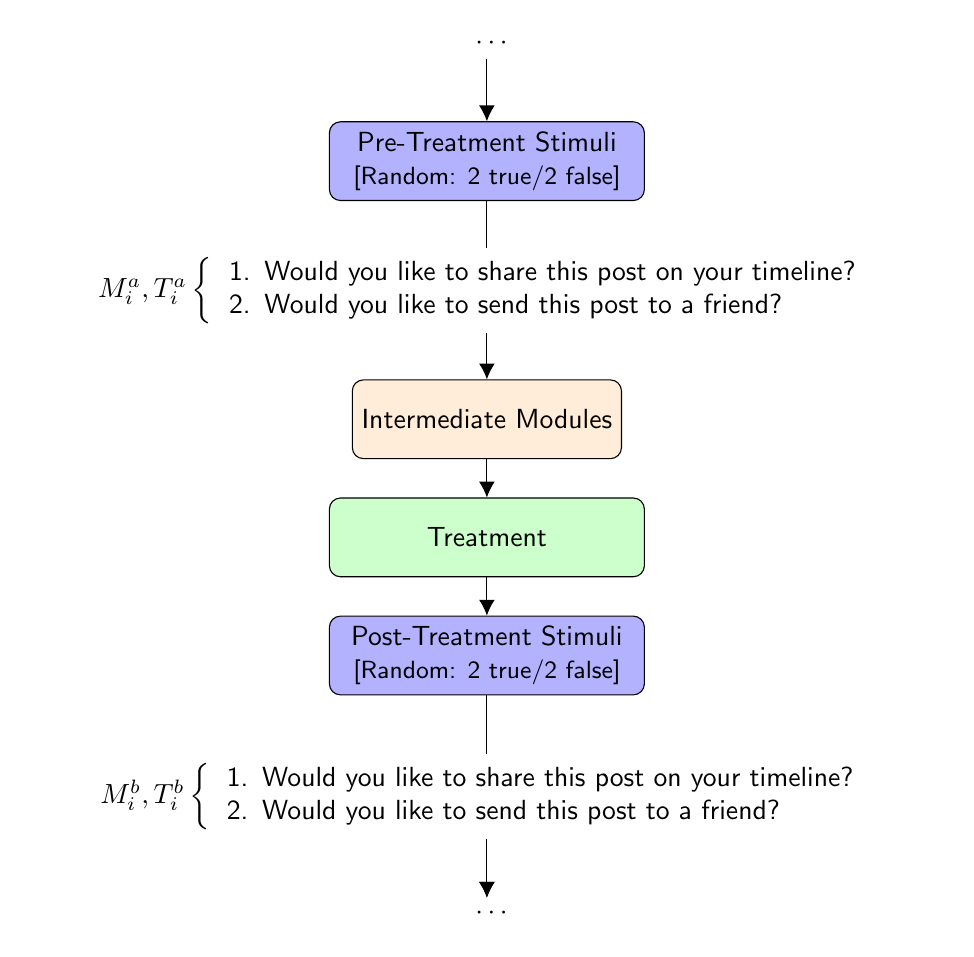
\begin{tikzpicture}[node distance=1.5cm,
    every node/.style={fill=white, font=\sffamily}, align=center]
  % Specification of nodes (position, etc.)
 \node (pre)      [draw=none,rectangle, fill=none]
                                                      {\ \ $\cdots$ };    
 \node (pretreat)             [activityStarts, below of = pre]              {Pre-Treatment Stimuli \\ \small{[Random: 2 true/2 false]}};
  \node (distract)      [process, below of=pretreat, yshift=-.7in]
                                                      {Intermediate Modules};
  \node (treat)      [activityRuns, below of=distract]
                                                      {Treatment};
  \node (posttreat)      [activityStarts, below of=treat]
                                                      {Post-Treatment Stimuli \\ \small{[Random: 2 true/2 false]}};  
  \node (etc)      [below of=posttreat, yshift=-.7in, draw=none,rectangle, fill=none]
                                                      {\ \ $\cdots$ };    
    \draw[->]             (pre) -- (pretreat);    
     \draw[->]             (pretreat) -- node[text width=4.5in]
     				{
                                                $M_i^a, T_i^a
                                                \left\lbrace
                                                \begin{tabular}{ l} 
                                                1. Would you like to share this post on your timeline?\\
                                                2. Would you like to send this post to a friend?
                                                \end{tabular}\right.
                                                $
						 }(distract);
     \draw[->]             (distract) -- (treat);    
     \draw[->]             (treat) -- (posttreat);       
     \draw[->]             (posttreat) -- (etc);                      
     \draw[->]             (posttreat) -- node[text width=4.5in]
                                   {
                                                $M_i^b, T_i^b 
                                                \left\lbrace
                                                \begin{tabular}{ l} 
                                                1. Would you like to share this post on your timeline?\\
                                                2. Would you like to send this post to a friend?
                                                \end{tabular}\right.
                                                $
                                                }(etc);
\end{tikzpicture}
\end{figure}
%\end{document}

Prior to treatment, we show respondents four media posts from their country (two true and two false in random order) randomly sourced from our stimuli set. For each stimuli we ask the above self-reported sharing intention questions (see Figure \ref{survey_flow}). Respondents are then asked a series of questions about their media consumption, and are then randomly assigned treatment according to the experimental design. If assigned to one of the respondent-level treatments, they are administered the relevant treatment. They are then shown four additional stimuli (two true and two false), selected from the remaining stimuli that they were \textit{not} shown pre-treatment. If the respondent is assigned a headline-level treatment, this treatment is applied only to the misinformation stimuli, as flags and fact-checking labels are not generally applied to true information from verified sources. For each of the stimuli we again ask the same self-reported sharing intention questions. 

We code response to the self-reported questions as one if the respondent affirms they want to share the post and zero otherwise. Let $M_i^a$ be the sum of respondent $i$'s pre-test responses to the \textit{misinformation} stimuli and let $T_i^a$ be the sum of respondent $i$'s pre-test responses to the \textit{true} informational stimuli. $M_i^b$ and $T_i^b$ are the respective post-treatment responses. Then $M_i^a, T_i^a, M_i^b, T_i^b \in \{0,1,2, 3, 4\}$. 

We control for strata of pre-test responses in our analyses.\footnote{{We measure strata separately by stimuli type and by channel, for a total of \{(True, False)\}$\times$\{(timeline, Messenger)\}$\times$\{0:2 response values\} = 12 strata indicators.}}
We formalize our response function in terms of post-test measures:
\[
Y_i = -M^b_i + 0.5 T^b_i.
\]
This response function is the metric that we optimize for in our adaptive algorithm described in Section~\ref{adaptiveagent}, and in our policy learning described in Section~\ref{analysis}. Because of random assignment, we expect to see no systematic differences in pre-test interest in sharing either true or false stimuli across treatment conditions, conditional on covariates. 


As shown in Table \ref{tab:response_fun}, {the highest value is achieved when users share all true stimuli, both through messenger and on their timeline ($T^b_i = 4$) but share no misinformation ($M^b_i = 0$). The lowest value is achieved in the reverse scenario, sharing all false but no true information. Along the diagonal, when respondents share the same amount of true and false information, the value of $Y_i$ is decreasing with the number of pieces of misinformation shared to reflect the fact that someone who shares one true and one false stimuli is spreading \textit{less} misinformation, overall, compared to another who is sharing two true and false stimuli.}  


% response function table in case we want it
\begin{table}[!ht]
\centering
\begin{tabular}{lrrrrrr}
                                   & \multicolumn{1}{l}{}   & \multicolumn{1}{l}{} & \multicolumn{1}{l}{} & \multicolumn{1}{l}{\textbf{$T_i$}} & \multicolumn{1}{l}{} & \multicolumn{1}{l}{}      \\ \cline{3-7} 
                                   & \multicolumn{1}{r|}{}  & 0                    & 1                    & 2                                 & 3                    & \multicolumn{1}{r|}{4}    \\ \cline{2-7} 
\multicolumn{1}{l|}{}              & \multicolumn{1}{r|}{0} & 0.0                  & 0.5                  & 1.0                               & 1.5                  & \multicolumn{1}{r|}{2.0}  \\
\multicolumn{1}{l|}{}              & \multicolumn{1}{r|}{1} & -1.0                 & -0.5                 & 0.0                               & 0.5                  & \multicolumn{1}{r|}{1.0}  \\
\multicolumn{1}{l|}{\textbf{$M_i$}} & \multicolumn{1}{r|}{2} & -2.0                 & -1.5                 & -1.0                              & -0.5                 & \multicolumn{1}{r|}{0.0}  \\
\multicolumn{1}{l|}{}              & \multicolumn{1}{r|}{3} & -3.0                 & -2.5                 & -2.0                              & -1.5                 & \multicolumn{1}{r|}{-1.0} \\
\multicolumn{1}{l|}{}              & \multicolumn{1}{r|}{4} & -4.0                 & -3.5                 & -3.0                              & -2.5                 & \multicolumn{1}{r|}{-2.0} \\ \cline{2-7} 
\end{tabular}
\caption{Table of response function values ($Y_i$)}
\label{tab:response_fun}
\end{table}



{In the study of misinformation sharing, there are a number of ways that we could formalize our response function. For instance, we could design a study that is only concerned with the sharing of \textit{false} information, without any attention to rates of sharing \textit{true} information. Favoring this kind of response function, however, would not distinguish between treatments that simply reduce sharing overall. Particularly since we are interested in policy-relevant and operational treatments, we favor an approach that takes into account the sharing of true \textit{and} false information since we are interested in the overall media environment on social media platforms.} This design follows existing studies that similarly focus on the ratio of true-false information sharing \citep{jahanbakhsh2021exploring}.

{Here we also pool across sharing modes (timeline and messenger) in our response function. While of course these different sharing channels likely have different implications for audience reach and impact, we did not want to make a judgment as to which poses a more serious threat overall. For example, one might argue that posting misinformation on the Facebook timeline is more dangerous since it is public to friends and would therefore reach more users, compared to a private message. The counterargument to prioritizing the reduction in timeline posts is that users might take timeline posts less seriously than a private message that is individually sent from a friend. For these reasons, and for ease of interpreting our response function, our response function values both timeline and messenger sharing equally. After data collection, however, we will also analyze timeline and messenger sharing outcomes separately to observe any differences in treatment effectiveness with respect to the mode of sharing.
}

{Based on our pilot data, it became clear that some individuals may share fact-checked stories with warning labels out of a desire to share the \textit{correction} with their friends who, for instance, may have believed that alcohol could help prevent COVID-19. To gather data on users' motivations for sharing in a realistic way, we include a follow-up question after the \textit{last} stimulus that the respondent views. After the respondent answers our two main outcome measures of interest for the last stimulus if they indicate wanting to share the story through either channel, they are then prompted to: ``Please write the message you would like to include with your [messenger/timeline] post.'' They are free to write any message they wish, as they would if they were really sharing the story. We include an additional stimulus of the opposite type (True/False) as the last stimulus, so that we can collect responses on motivation for sharing for both true and false stimuli. We include this follow-up prompt only for the last headline and a bonus stimulus, so as not to prime and affect inputs to our primary response function. We will have a research assistant hand code these open text responses to get a better sense of underlying motivations to share false information and how these warning flags are understood. 
} 


\subsubsection{Secondary Outcomes}
Additionally, we measure secondary behavioral outcomes which allows us to further investigate the extent to which treatments may suppress the sharing of \textit{true} information.

In order to obtain a behavioral measure of sharing, we collect the articles the respondent indicated they would like to share throughout the survey and at the end of the survey provide links to the \textit{true} information. For these true stimuli, we offer respondents the opportunity to actually share this information as a Facebook post, which has been created on our project Facebook page. We are able to measure whether respondents click on a button which opens a pop-up screen to share the post on Facebook, however, we cannot directly fully measure whether they then actually follow through to the second step and post the article on their own timeline, as this information is not available to us for individuals who do not make the post public. Consequently, we report only rates of clicking the initial share button. The response function here is measured as the percent of true stimuli that the respondent said they wanted to share during the survey for which they later click the button to share on Facebook. (We do not differentiate between stimuli presented pre- and post- treatment here, since the behavioral response measurement for all stimuli is all post-treatment.) To provide some insight into the extent to which respondents followed up on an intention to share, we report the \textit{aggregate} number of times the associated post for each stimuli was shared. 

At this point we also debrief respondents, informing them about the headlines they were shown that are false. Instead of allowing respondents to share these headlines, we provide links to tips for spotting misinformation online; we measure click-through-rates for these links as well. 


\subsubsection{Attrition} We will include in analysis all respondents for whom we have collected complete pre-test responses. As treatment is not revealed at this point, attrition should be independent of treatment assignment conditional on covariates. For respondents who attrit after collection of pre-test responses and before collection of post-test responses, the post-test interest in sharing response function will be coded as identical to the individual pre-test value; for behavioral sharing outcomes, we impute zeros for click-through-rates.\footnote{An alternative approach to analysis in a pre-test/post-test design, accounting for missing data, would be to follow \cite{davidian2005semiparametric}'s implementation of estimators developed by \cite{robins1994estimation}.}

{Just before respondents receive the treatment we include a very simple attention check, which asks respondents to reenter their age. In the pilot, less than 3\% of users failed this check. We will include all respondents, even those who failed this attention check, in the main analysis but also include an indicator variable for whether respondents failed this check as a covariate used for prediction in our conditional means model used to estimate doubly robust scores.} %LR: not sure removing them necessary but can keep for good measure

\subsubsection{Follow-Up Survey}

In evaluating experimental techniques to curb the influence and spread of misinformation, researchers most often measure outcomes only moments after the treatment is delivered. Yet, in designing policy interventions to combat misinformation it is critical to understand not only whether a particular invention is immediately effective, and which policy is optimal, but also for how long a given treatment is effective. We therefore plan to conduct follow-up surveys to investigate the duration of treatment effects. Specifically, we will send a follow-up survey that includes just two stimuli (not viewed during the main survey) and again ask respondents whether they want to share either of these stories through messenger or on their timeline. Half of the sample will be randomly assigned to receive the follow-up one day after the end of the main survey. The other half will be sent the follow-up three days after the end of the main survey. The main data collection is estimated to take approximately ten days, in which case respondents will receive the follow up survey anywhere from one day to about two weeks after their original survey. Using these outcome measures collected at a later date, we will be able to examine treatment decay over time. Following \citet{broockman2017design}, we will analyze duration effects adjusting for differential response rate to the follow-up survey and the number of days since the respondent completed the survey.  
 

\section{Hypotheses and Data Collection}

Our data is described by treatments $W_i \in \ww$\footnote{Our treatments are composed of two separate factors, but here we use $W$ to represent combined treatment conditions, i.e., the unique combination of one respondent-level and one headline-level treatment. Where we wish to explicitly differentiate, we use $W^R_i$ and $W^H_i$ for respondent- and headline-level treatments respectively. Each factor includes a baseline level absent intervention, and the cardinality $|\ww| = |\ww^H|\times |\ww^R|$.}; response,  $Y_i \in \RR$; and covariates, $X_i \in \xx$. 

The data is indexed by $i = 1, \dots, N$ where indexing represents the order in which respondents entered the experiment; this allows us to use $i$ to also represent relative chronological relationships in our sequential adaptive design. 

We use potential outcome notation, where $Y_i(w)$ represents the potential outcome for respondent $i$ under treatment $w$.


We would like to learn and evaluate policies, under which we assign the most effective treatment conditional on covariates. Formally, a policy maps a set of covariates to a decision \citep{athey2021policy},
\begin{align}
  \pi: \xx \rightarrow \ww. 
  \label{eq:policy}
\end{align}
Although the definition allows for a policy to be contextual, it need not be; below, we will also consider the best uniform policies for each of our different types of interventions. In our setting, we will learn the policy, $\hat \pi$, and evaluate its value. The value of a policy is defined as, 
\begin{align}
V(\pi) =  \E[Y(\pi(X_{i}))],
  \label{eq:policy_value}
\end{align}
where the expectation is taken over the distribution of $X$.\footnote{Here we will only consider deterministic policies, but for a random policy, the expectation will be taken over the joint distribution of the covariates with the policy. }

\subsection{Hypotheses}\label{hypotheses}

\subsubsection{Optimal uniform and contextual policies}\label{policiesbest}
Our hypotheses of interest are with respect to the value of an estimated optimal contextual policy $\pi_{opt}$, and fixed policies $\pi_{W}$, where under each fixed policy we would assign all respondents the relevant treatment $w$. The pure control policy is the fixed policy $\pi_{c}$ where both respondent and headline-level factors are set to the baseline control condition. 

\paragraph{Uniform policies}
{We learn the best uniform respondent and headline-level policies from the data, and for each of these uniform policies, test whether they improve response over the control policy.}
\setcounter{hypothesis}{1}
  \begin{subhyp}
  The best uniform headline-level policy, i.e., the fixed headline-level treatment with the highest associated value, improves response over the control policy. 
  \label{eq:headlinectr}
\begin{align}
  H_{0}: \max_{w^H} V(\pi_{W^H}) = V(\pi_{c}) \qquad H_{a}:  \max_{w^H} V(\pi_{W^H}) > V(\pi_{c})
\end{align}
\end{subhyp}

  \begin{subhyp}
  The best uniform respondent-level policy, i.e., the fixed respondent-level treatment with the highest associated value, improves response over the control policy. 
  \label{eq:respondentctr}
\begin{align}
  H_{0}: \max_{w^R} V(\pi_{W^R}) = V(\pi_{c}) \qquad H_{a}:  \max_{w^R} V(\pi_{W^R}) > V(\pi_{c})
\end{align}
\end{subhyp}

\paragraph{Contextual policy}
As well, we test whether we are able to estimate from the data an optimal contextual policy that improves value over the control. When we consider power of our experiment in simulations, we focus on this hypothesis, as we are \textit{most} interested in the policy that is \textit{most} effective at moving our response function, and the contextual policy should be weakly superior to both the uniform respondent and headline-level policies. 
  \begin{hypothesis}
  The best contextual policy that can be estimated from the data achieves higher value than the control treatment. \label{eq:optctr}
\begin{align}
  H_{0}: V(\pi_{opt}) = V(\pi_{c}) \qquad H_{a}:  V(\pi_{opt}) > V(\pi_{c})
\end{align}
\end{hypothesis}

We would also like to learn how much we gain by exploiting heterogeneity in the data. As secondary hypotheses, we propose that the optimal policy that we are able to estimate from the data improves over the best uniform respondent and headline level treatments; we learn these best uniform policies from the data, and test these hypotheses separately. 
\setcounter{hypothesis}{2}
  \begin{subhyp}
  The best contextual policy that can be estimated from the data achieves higher value than the best uniform headline-level treatment, i.e., the fixed headline-level treatment with the highest associated value. 
  \label{eq:optheadline}
\begin{align}
  H_{0}: V(\pi_{opt}) = \max_{w^H} V(\pi_{S^H}) \qquad H_{a}:  V(\pi_{opt}) > \max_{w^H} V(\pi_{W^H})
\end{align}
\end{subhyp}

  \begin{subhyp}
 The best contextual policy that can be estimated from the data achieves higher value than the best uniform respondent-level treatment, i.e., the fixed respondent-level treatment with the highest associated value. 
\begin{align}
  H_{0}: V(\pi_{opt}) = \max_{w^R} V(\pi_{W^R}) \qquad H_{a}:  V(\pi_{opt}) > \max_{w^R} V(\pi_{W^R})
\end{align}
\end{subhyp}

We discuss how we \textit{learn} these policies in Section~\ref{adaptivelearning}. 


\subsubsection{Further analyzing heterogeneity}\label{policieshte}

While our main goal is to learn and evaluate the policies that are most effective at moving our response, we have also designed the study to facilitate further exploration of heterogeneity. At a first level, we are interested in heterogeneity in response; do different subgroups respond differently? For example, do we see that older respondents have higher responses on average than younger respondents?

We note that heterogeneity in response does \textit{not} necessarily imply treatment effect heterogeneity -- for example, if older respondents have consistently higher responses under both the accuracy nudge and control, we will not find treatment effect heterogeneity here. Along similar lines, significant treatment effect heterogeneity does not necessarily imply that we will learn a contextual policy that improves value over a uniform policy. In our pilot, the respondent-level accuracy nudge treatment \citep{pennycook2020fighting} appears to be most effective overall, so let's assume that this is the best uniform policy. Suppose we see treatment effect heterogeneity such that older respondents respond better to the Facebook tips compared to the AfricaCheck tips, whereas the reverse is the case for younger respondents. For us to uncover a meaningful contextual policy using these subgroups and treatments, one of these treatments needs not only to be more effective than the other for a given subgroup, but more effective than the accuracy nudge.

%% My attempt at above par. in simpler language:
% do subgroups respond differently to diff treatments -- e.g. do older/younger users respond differently to our diff treatments
% It could be, for instance, that the accuracy nudge treatment is the best uniform respondent-level treatment -- and that this has HTE --> is more effective among young than old. BUT this is different from finding that, for instance, among a certain subgroup the HTE is to such a degree that actually there is a different policy that achieves a higher value for this particular subgroup than even the best uniform resp-level treatment. On the other hand, it could be that we find heterogeneity here but not to the degree that there is a different policy that does better for a particular group.
%% might be useful in general to lean on the plots below and use concrete examples based on these data?


{In Figure}~\ref{fig:science_crt}{, we provide examples of variation among best respondent-level treatment conditions from our pilot data, comparing the respondent-level interventions that are most effective for certain subgroups to the control. We selected the given cross-tabs based on preliminary analysis from the pilot, but we are not powered to rigorously evaluate differences in response in these sub-groups with these data, and so these examples are for illustration and theory-generation only. See Table}~\ref{cov_long} {in Appendix}~\ref{appendix:covariates} {for definition of covariates and description of indices. }

{We expect the accuracy nudge to be most effective for the plurality of individuals, who may simply not be very attentive as they share information online.} {In the top panel of Figure}~\ref{fig:science_crt}{, we consider variation for older and more technologically savvy individuals, as measured by being above median age and digital literacy index (DLI). We propose that these respondents will be more responsive to treatments that provide more information, such as the fact-checking training treatments. We see that for both younger and older respondents with low DLI, the accuracy nudge remains the best overall treatment. For younger respondents with high DLI, the Facebook tips are most effective; for older respondents with high DLI, Facebook tips out-perform the accuracy nudge, but the control condition is overall the most effective. }

{In the lower panel of Figure}~\ref{fig:science_crt}{, we consider variation based on scientific views and cognitive reflection test, as measured by being above median for our scientific views index and cognitive reflection test (CRT). We see that for individuals with less scientific views, whether their CRT is high or low, the accuracy nudge remains the best overall treatment. For those with highly scientific views and low CRT scores, the AfricaCheck tips are most effective; for those with highly scientific views and high CRT scores, the video treatment is most effective. }

\begin{figure}[H]
\centering
\includegraphics[width=\textwidth]{figures/age_dli.pdf}
\includegraphics[width=\textwidth]{figures/science_crt.pdf}
\caption{Examples from the pilot of heterogeneity in \textit{best} respondent-level treatment. Note that in our pilot data we are not well-powered to evaluate these differences, and so these examples are for illustration only. }
\label{fig:science_crt}
\end{figure}\FloatBarrier


{Based on this preliminary analysis of the pilot data, we hypothesize that there will be a subgroup of  ``attentive users'' who are likely to have high digital literacy scores, high cognitive reflection test (CRT) scores, and high scientific knowledge for whom the accuracy nudge \textit{will not} be the optimal contextual policy because these types of users are generally already considering the accuracy of a headline before they share it. For this subgroup, we anticipate that reminding users of additional ways to spot misinformation (e.g., the Facebook/AfricaCheck tips and video training treatments) will be the optimal policy. To evaluate this hypothesis, we will reproduce the above plots using data from the main study. We will also use data-driven techniques, specifically generalized random forests, to examine the composition of subgroups for whom the optimal contextual policy diverges from the best uniform policy.}


{In the below hypotheses, we focus on heterogeneous response, to better understand the sources of variation that will lead to heterogeneous treatment effects and effective contextual policies.} 

\paragraph{Hypotheses to inform industry practice:}
We select the below treatments because these are currently, or were previously, used by social media companies including Facebook and Twitter. The below covariates were selected as those that social media companies directly collect or have access to, and therefore could more easily use for targeting interventions. For our covariates of interest we will divide these into two groups for any binary variables (i.e. indicator for male) and split on the median value for continuous variables to test two subgroups (i.e. age $\geq$ median and age $<$ median). 

\textbf{Treatments:}
\begin{itemize}
\item Facebook tips (respondent)
\item AfricaCheck tips (respondent)
\item Factcheck (headline)
\item More information (headline)
\item Related articles (headline)
\end{itemize}

\textbf{Covariates:}
\begin{itemize}
\item Age
\item Male
\item Education
\end{itemize}

We hypothesize that the three headline-level treatments listed above will perform better among more educated users, older people, and among women, compared to the less educated, younger and male respondents. We expect that the two respondent-level treatments will reduce sharing of misinformation more among less-educated respondents than those with more education. 

\paragraph{Hypotheses to inform social science theory:} Previous studies have hypothesized and tested the role that deliberation plays in mitigating belief and sharing of online misinformation \citep{bago2020fake,pennycook2020fighting}. Drawing on these findings, we anticipate that our \textit{accuracy nudge} and \textit{deliberation nudge} respondent-level treatments may help shift respondents from system I, intuitive reactions, to system II, more deliberative thinking by nudging respondents to stop and think about the accuracy of the headline, in the former, and about \textit{why} they share posts, in the latter. We anticipate that these treatments will perform comparatively better among respondents who score low on our CRT measure by getting these intuitive thinkers to stop and reflect. Alternatively, these treatments could perform best among high CRT respondents if they are better able to engage with these treatments in the desired way. 


% pledge hypotheses
We expect the pledge respondent-level treatment to be more effective among people who more frequently post and interact with friends on Facebook, those who are more religious (i.e. those who attend religious services more frequently), and those with high CRT scores. Among respondents who are randomly assigned the \textit{public} pledge treatment, we anticipate this treatment to be more effective among respondents who engage on Facebook regularly (as measured by the number of times they posted in the past 7 days and their frequency of communication with friends on the platform during the same period). In other words, we expect that people who are more engaged on social media, and therefore likely have more meaningful connections on the platform, will face higher audience costs to pledging to fight misinformation and then sharing dubious posts and will therefore reduce their sharing of misinformation. We also hypothesize that more religious respondents and those with high CRT scores, compared to their counterparts, may have stronger motivations to remain consistent with their own behavior. Meaning if they have pledged to help spot misinformation, they will be less inclined to share it -- at least compared to those who may care less about commitment and consistency with their own previous actions. We evaluate heterogeneity with respect to intention to treat, i.e., individuals who were assigned to the pledge treatment, irrespective of whether they actually took the pledge. However, we will also report rates at which respondents clicked the button to share the pledge across groups under comparison.


\paragraph{Best respondent and headline-level treatments:} In addition to the above hypotheses related to response heterogeneity, we also plan to test heterogeneity with respect to the best performing respondent-level and headline-level treatments. To estimate these we again take the median as the splitting point of continuous covariates to create ``high'' and ``low'' categories: 

Specifically, we will test:
\begin{enumerate}
\item How locus of control and age interact with the best uniform respondent-level treatment. 
\item How CRT and education interact with the best uniform headline-level treatment. 
\end{enumerate}


\paragraph{Baseline levels}\label{baseline_levels}
In addition to response heterogeneity, we also anticipate that certain types of people are simply more likely to share false information, compared to true information. In particular, we expect that baseline rates of sharing false posts (compared to true posts) will be higher among these subgroups:
\begin{itemize}
\item young
\item male
%\item high internal locus of control
\item less educated
\item low CRT
\item more religious
\end{itemize}


\subsection{Adaptive data collection}\label{adaptiveagent}

In our data collection, we use a \textit{contextual bandit} algorithm, in which we sequentially update treatment assignment probabilities based on the observed history of treatment, response, and covariates. These types of algorithms navigate a tradeoff in \textit{exploration} of the response surface with \textit{exploitation} of those treatments which we have observed to be effective based on historical data. This allows us to continue to learn about treatment effect heterogeneity while improving outcomes over time \textit{within} the frame of the experiment. 

We will use a version of linear Thompson sampling \citep{agrawal2013thompson}. Under Thompson sampling \citep{thompson1933likelihood,thompson1935theory}, treatment is assigned according to the Bayesian posterior probability that each treatment is best. In linear Thompson sampling, this is generalized to allow the outcome to be a linear function of covariates. Under this approach, we denote contexts associated with counterfactual potential outcomes as $x_{[w]}$, where $x$ is the observed covariate vector, augmented by the treatment indicator(s) consistent with treatment $W =w$, and potentially treatment covariate interactions; let this vector be of length $d$ for all $w \in \ww$. 

We implement the linear model supposing that there is some unknown coefficient vector $\theta\in R^{d}$, such that the $\E[Y_i(w)|X_i = x] = x_{[w]}^\top \theta$. %\sim \mathcal{N}\left( x_{[w],i}^\top \theta, \nu\right)$.%\footnote{Note that the variance term here is different than the coefficient variance covariance matrix discussed below. We follow \cite{agrawal2013thompson} in setting $\nu$ as a term that accounts for the sample size, the dimensionality of the covariates, and the variance or bounding of the distribution; we note that in this implementation, it does not vary across treatment arms.} 
We assign treatment under the heuristic that the reward distribution is Gaussian, but, as \cite{agrawal2013thompson} note, we do not require the true reward distribution to be Gaussian for regret bounds to hold. 

%We assume the variance is constant within arms, i.e., $\hat\V[Y(w)|X = x] = \sigma^2_w$. The conditional reward function is modeled as being distributed,
%  \begin{align}
%    \mu_w(x) \sim \mathcal{N}({\mu}_w(x), {\sigma}_w^{2}(x)) \qquad %\text{for } s \in \{1, \cdots, S\} \text{ and treatment }w
%    \text{ for all treatments }w \in \ww
%  \end{align}


Our implementation roughly follows the balanced linear Thompson sampling algorithm described in \cite{dimakopoulou2017estimation, dimakopoulou2019balanced}, where the estimates $\hat\theta$ and $\hat\V[\hat\theta]$ are produced using weights to account for unequal assignment probabilities. We use a batched approach to updating, collecting data and then updating the treatment assignment model after each batch. We denote batches $\mathcal{I}_b$ for $b = 1, \dots, B$. Full details for the batch-wise linear Thompson sampling algorithm are provided in Algorithm~\ref{algg:bblts}; we present an overview below. 

\paragraph{Adaptive agent}\label{agent}

\begin{enumerate}
\item In the first batch, $b = 1$, we assign treatment uniformly at random. 

\item For equally sized batches $b = 2, \dots, B-1$:

\begin{enumerate}
   \item \label{step:fit} At the beginning of each batch, fit a ridge regression of the outcome regressed on observed treatment-augmented covariates; compute the minimum mean cross-validated error value of the penalization factor $\lambda^{CV}$ using the entire observed history of data. 
    This model with penalty term $\lambda^{CV}$ produces our estimate of the coefficient vector $\hat \theta$ and variance, $\hat\V[\hat\theta]$.\footnote{
We use the below linear model for the length $d$ parameter vector $\theta$, 
\begin{align*}
\hat{Y}(W) | X & =
			\sum_{w^R} 1\{W^R = w^R\}\beta_{w^R}  +
			\sum_{w^H} 1\{W^H = w^H\}\beta_{w^H}  +\\ 
			& \sum_{w^R} \sum_{w^H}1\{W^R = w^R\} \times 1\{W^H =  w^H\}\beta_{w^{R,H}} +  \\
			& \sum_{\ell}  X_{[\ell]}{\beta}_{\ell} +\\
			& \sum_{w^R} \sum_{w^H}1\{W^R = w^R\} \times 1\{W^H =  w^H\}  X_{[\ell]} {\beta}_{w^{R,H}. \ell}.
			\numberthis
         \label{eq:linear_model_full}
\end{align*} 
The model is estimated using $L_{2}$ penalties for regularization, exclusive of the main treatment effects $\beta_{w^R}$ and $\beta_{w^R}$. 
Observations are weighted according to standard inverse probability weights using known assignment probabilities, following \cite{dimakopoulou2017estimation}, as in Equation~(\ref{eq:IPW}). 

We assume covariates are mean-centered and scaled to have sample variance of one \citep{marquardt1980you}; in practice, this re-scaling occurs each time we fit the ridge regression. 
}

For each observation $i$ in batch $b$,
\begin{enumerate}
 \item Draw $M=1,000$ draws from $\tilde \theta ^{(m)} \sim \mathcal{N}\left(\hat \theta,\hat\V[\hat\theta]\right)$, and calculate the proportion of times each arm produced the maximum estimate under the counterfactual treatment augmented covariate profile  $x_{[w]i}$:
				\begin{align}
   q_w = \frac{1}{M} \sum_{m=1}^M 1\left\{ w = \underset{w}{\argmax} \{ x_{[1]i}^\top \tilde \theta ^{(m)}, \dots, x_{[|\ww|]i}^\top\tilde \theta^{(m)} \}  \right\}
				\end{align}
	These are the raw Thompson sampling probabilities. 	
\item In our algorithm, these probabilities are constrained by a pre-determined probability floor, $p$, and rescaled to sum to one, giving us $e_{1}, \dots, e_{|\ww|}$. 
\item Assign treatment  according to the calculated probabilities: \\
$w_i \sim \textrm{Multinom} \left( e_{1}, \dots, e_{|\ww|} \right)$
\end{enumerate}
\end{enumerate}

\item For the final batch,  $b = B$, learn policies and collect data for evaluation. 

At the beginning of the batch, 
\begin{enumerate}
  \item Fit an optimal contextual policy, and learn the best uniform headline-level policy and the best uniform respondent-level policy. Approaches to learning these policies are described in Section~\ref{analysis}, below. 
  \item For each observation $i$ in the final batch, assign treatment with equal probability to:\label{step:policies}
  \begin{itemize}
  \item the pure control, 
  \item the best uniform headline level policy, with no respondent-level treatment, 
  \item the best uniform respondent-level policy, with no headline-level treatment, and
  \item the best contextual policy conditional on $x_i$. 
  \end{itemize}
\end{enumerate}
\end{enumerate}


\section{Analysis}\label{analysis}

To learn the best uniform and contextual policies, we must conduct a preliminary evaluation on the adaptively collected data. We then use the last batch for final evaluation and hypothesis testing. To account for unequal treatment assignment probability, we use doubly robust scores $\Gamma_{i,w}$, as in (\ref{eq:DR}), following \cite{robins1994estimation}'s augmented inverse-propensity weighted scores, 

      \begin{align*}
        \Gamma_{i,w} = \mu_{w}(X_{i}) + 1 \{W_i = w \} \xi_w(X_i)(Y_{i} - \mu_w(X_i)), \numberthis\label{eq:DR}\\
         \mu_{w}(x)  = \E[Y_i(w) | X_i = x].
    \end{align*}

We estimate $\hat\mu_{w}(X_{i})$, the conditional mean for each $w$ using generalized random forests, as implemented by the \texttt{grf} package in \texttt{R} \citep{Tibshirani:2020aa}. 
$\xi_w(X_i)$ is a weight to account for unequal treatment assignment probabilities. {Again, we can use the full covariate set, as described in Appendix}~\ref{appendix:covariates}{, including the pre-test response measures on the righthand side of the model.}
We use inverse probability weights, 
\begin{align*}
\xi^{IPW}_w(X_i) = \frac{ 1 }{e_{w}(X_i)}, \label{eq:IPW} \numberthis\\
e_{w}(x) = \Pr[W_i = w|X_i = x].
\end{align*}
Here, we can directly plug in the respective treatment assignment probabilities from the experimental design for the $e_{w}(X_i)$. 
 

\subsection{Policy learning and evaluation on adaptively collected data}\label{adaptivelearning}

\begin{enumerate}
\item \textbf{Compute doubly robust scores}. For adaptively collected data, we use doubly robust scores as in (\ref{eq:DR}), but due to the dependent nature of the data, to avoid bias, we must ensure that we use only historical data in our estimates of the nuisance components. \label{step1}

The weights $\xi^{IPW}_w(X_i)$ are by design only produced from historical data. To estimate conditional means $\hat \mu_w(X_i)$, for each batch $b$ in $b = 1, \dots, B-1$ and for each treatment $w$:
\begin{enumerate}
\item Fit a random forest estimator on the observations assigned $w$ in batches up to and including batch $b$. 
\item For observations assigned $w$ in batch $b$, calculate $\hat\mu_w(X_i)$ using out-of-bag predictions. 
\item For observation \textit{not} assigned $w$ in batch $b$, calculate $\hat\mu_w(X_i)$ using regression forest predictions from the fitted model in step a. 
\end{enumerate}

 Compute doubly robust scores $\hat{\Gamma}_{i,w}$ plugging the estimated nuisance components into (\ref{eq:DR}). 
\item \textbf{Learn policies}. We learn policies on the data collected up to batch $B-1$, by taking the average of scores over the relevant evaluation sets $\mathcal{I}$, where $\mathcal{I}_b$ represents the set of all observations within batch $b$.
\begin{enumerate}
  \item Learn fixed policies on the adaptively collected data. 
      \begin{align}
          \hat{V}({\pi}_{w})  &:= \frac{1}{\bigg{\lvert} \bigcup\limits_{b=1}^{B-1} \mathcal{I}_{b} \bigg{\rvert}} \sum_{i \in \bigcup\limits_{b=1}^{B-1} \mathcal{I}_{b} } \hat{\Gamma}_{i,w}
        \end{align}  
   To learn the \textbf{best uniform headline-level policy}, we average over all treatment combinations that include a given headline treatment; effectively, this marginalizes over a balanced distribution of the respondent-level policies. {When we evaluate this policy, however, we will implement} \textit{{only}}{ the uniform version of the policy, i.e., with no corresponding respondent-level policies. }
      \begin{align}
                          \hat{V}({\pi}_{w_H})  &:= \frac{1}{\bigg{\lvert} \bigcup\limits_{b=1}^{B-1} \mathcal{I}_{b} \bigg{\rvert}} \sum_{i \in \bigcup\limits_{b=1}^{B-1} \mathcal{I}_{b} } \bar{\Gamma}_{i,w_H} \\ %, \ \ w \ni w_H \\
w_H^* & =  \argmax_{w_H} \  \hat{V}({\pi}_{W_H})
\intertext{ The procedure is equivalent for learning the \textbf{best uniform respondent-level policy.}}
          \hat{V}({\pi}_{w_R})  &:= \frac{1}{\bigg{\lvert} \bigcup\limits_{b=1}^{B-1} \mathcal{I}_{b} \bigg{\rvert}} \sum_{i \in \bigcup\limits_{b=1}^{B-1} \mathcal{I}_{b} } \bar{\Gamma}_{i,w_R} \\%, \ \ w \ni w_R  \\
w_R^* & =  \argmax_{w_R} \  \hat{V}({\pi}_{W_R})
%\intertext{For the \textbf{best contextual policy}, we average scores }
%                     \hat{V}(\hat{\pi}_{opt})  &:= \frac{1}{\big{\lvert}  \mathcal{I}_{B} \big{\rvert}} \sum_{i \in \mathcal{I}_{B} }
%          \langle \hat{\pi}^*_{X_i}, \hat{\Gamma}_{i, \cdot} \rangle
    \end{align}
%   \item To learn and evaluate the best fixed policy on a dataset, we again take the relevant approach described in Appendix~\ref{appendix:bestfixed}. 
    \item For the optimal contextual policy, estimate a random forest model on the entire learning portion of the experiment, as described in Step~\ref{step1} above. We use a {point-wise optimal random forest policy,} where for each observation we will predict response under each unique treatment, and take the maximum.
        \begin{align*}
%            \hat{\pi}_{opt} = \arg\max_{\pi \in \Pi}
%            \langle \pi(X_{i}), \hat{\Gamma}_{i, \cdot} \rangle \\
%            \text{where } \Pi \text{ is the class of depth-\textcolor{black}{two} policy trees.}\\
%            OR \\
            \hat{\pi}_{opt}(x_i)  =     \argmax_{w}
            \hat{\mu}_{w}(x_i) \\
             \text{where }\hat{\mu}_{w} \text{ is the random forest model.}
        \end{align*}
%    To ensure we learn an optimal policy that is contextual, if we learn a policy in which the policy tree recommends all actions that are equivalent across leaves (i.e., the policy is not contextual), we remove this fixed treatment and re-learn the tree policy on the remaining treatments; we repeat this until we learn a non-uniform policy. 
\end{enumerate}
\item \textbf{Evaluate policies} We hold out the last batch of data for policy evaluation and hypothesis testing. This allows us to learn and evaluate policies on separate splits of the data, whereas we otherwise would be subject to bias in our policy evaluations from over-fitting. Additionally, when using adaptively collected data, we are not able to use standard cross-fitting techniques such as k-fold cross-validation, due to the temporal dependencies. We conduct policy evaluation simply by estimating doubly robust scores, and then average scores under the policy of interest over the last batch of the experiment. 

The procedures for estimation on data collected using simple random assignment, as in the pilot and some simulations below, are described in Appendix~\ref{randomlearning}, but are parallel to the steps outlined above. %We again estimate nuisance components and compute doubly robust scores using only the last batch of the data. Note that in this last batch, we have just four policies of interest, as described in Step~\ref{step:policies} of the \hyperref[agent]{Adaptive Agent}. 
\end{enumerate}
The data collected from this study may be used for eventual application of a contextual implementation of the evaluation weighting method proposed in \cite{hadad2019confidence}, and advanced for contextual cases in \cite{zhan2020retrospective}. However, these methods will not be discussed in this pre-registration. 

Due to sampling variation, there may be some difference in covariate distributions between the last bast and prior batches, particularly as our covariate space has relatively high dimension. To account for this, we will also present results of analysis weighting by the inverse probability of appearing in the last batch, as predicted by a regression forest.


\subsection{Hypothesis testing and other analysis}
To evaluate the hypotheses from Section~\ref{hypotheses}, we estimate means and standard errors of the (differences in) policies using the averages and standard deviations of the (differences in) relevant scores, and conduct frequentist hypothesis testing. 

For analysis regarding main effects and heterogeneity with respect to the best contextual and best uniform respondent- and headline-level policies, we use only the last batch of the data. %, calculating doubly robust scores as described in Appendix~\ref{randomlearning}. 

For analysis regarding main effects and heterogeneity with respect to pre-determined factor levels, we use the adaptively collected data up through batch $B-1$, calculating doubly robust scores as described in Section~\ref{adaptivelearning}. When considering a specific factor level, we marginalize over a balanced distribution of the other factor.\footnote{For example, if we are interested in average outcomes under the Pledge respondent-level treatment, we will take an average of scores for the Pledge treatment crossed with each of the headline-level treatments, including the baseline control.} %
We note that this is different from the realized distribution of the other factor, as the adaptive design is intentionally unbalanced--and distributions of the \textit{other} factors will vary from level to level. We calculate these quantities by averaging across the relevant scores, and taking the standard deviations of the averages. 

\subsubsection{Main effects of each factor level}\label{main}
For the primary response function as well as secondary outcomes discussed in Section~\ref{response}, we report average outcomes under each headline factor level and separately each respondent factor level, marginalizing over a balanced distribution of levels of the other factor.

\subsubsection{Treatment effect heterogeneity}
The optimal contextual policy will allows us to describe subgroups across which the best intervention varies. We report the means and standard deviations of all covariates in each subgroup in the evaluation stage of the data. Comparing the differences in covariate distributions across subgroups can provide further insight into what may predict heterogeneous responses to treatment. 

To test hypotheses regarding specific heterogeneous response, as described in Section~\ref{policieshte}, we again average across the relevant scores, and compare estimates across the two groups. Given that testing these treatment-covariate combinations will result in a large number of unique tests, we will adjust for multiple hypothesis testing for response heterogeneity by reporting tests under both Bonferroni and Benjamini-Hochberg corrections for each set of hypotheses.



%\subsection{Conditional means model}\label{ridge}
%For the primary response function as well as secondary outcomes discussed in Section~\ref{response}, we report coefficient estimates from  a factorial conditional means model, where we conduct variable selection for interaction terms, and then conduct inference on the selected model (similar to the covariate-selection approach proposed by \citealt{bloniarz2016lasso}).  We use the following formulation in the variable selection model:
% 
%\begin{align*}
%\hat{\mu}_w(X_{i}) & =
%			\sum_{w^R} 1\{W^R_i = w^R\}\hat\beta_{w^R}  +
%			\sum_{w^H} 1\{W^H_i = w^H\}\hat\beta_{w^H}  +\\ 
%			& \sum_{\ell}  X_{[\ell]i}\hat{\beta}_{\ell} +\\
%			& \sum_{w^R} \sum_{w^H}1\{W^R_i = w^R\} \times 1\{W^H_i =  w^H\}\hat\beta_{w^{R,H}}. %+  \\
%			& \sum_{w^R} \sum_{w^H}1\{W^R_i = w^R\} \times 1\{W^H_i =  w^H\}  X_{[\ell]i} \hat{\beta}_{w^{R,H}. \ell}.
%			\numberthis
%         \label{eq:linear_model_full}
%\end{align*} 
%
%\begin{align*}
%\hat{\mu}_w(X_{i}) & =
%			\sum_{w} 1\{W_i = w\}\hat\beta_{w}  +
%			\sum_{\ell}  X_{[\ell]i}\hat{\beta}_{\ell} +
%			\sum_{\ell} \sum_{w}1\{W_i =  w\}  X_{[\ell]i} \hat{\beta}_{w, \ell}.\numberthis
%         \label{eq:linear_model_full}
%\end{align*} 
%The variable selection model uses $L_{1}$ penalties for regularization, exclusive of the main treatment effects $\beta_{w^R}$ and $\beta_{w^H}$. The OLS model includes only main effects and interaction terms. The models are estimated on the data from batches up to $B-1$. Covariates are mean-centered and scaled to have sample variance of one \citep{marquardt1980you}. Observations are weighted by their inverse probability weights, following \cite{vanderweele2010marginal}. %; regularization is hierarchically constrained over two levels of penalties, so that the penalty on covariate coefficients, the $\hat{\beta}_{\ell}$ terms, is less than or equal to the penalty on interaction of treatments or interaction of treatment with covariates, the $\hat\beta_{w^{R,H}}$ and $\hat{\beta}_{w^{R,H}, \ell}$ terms.  


\section{Simulations and design hyperparameters}\label{simulations}

This section documents our approach to making data-driven design decisions. To carry out implementation, the above description requires setting of several design hyperparameters, including total experiment size $N$, number of batches $B$,  size of first batch $|\mathcal{I}_1|$, size of last batch $|\mathcal{I}_B|$, and probability floor $p$. 

We set these hyperparameters by learning from our pilot data of approximately 1,500 observations from each country. We conduct the below simulations \textit{jointly} for the two countries.

\subsection{Simulation design}
\paragraph{Data generating processes} 

We simulate data generating processes (DGPs) based on the pilot data, with varying heterogeneity. We create these DGPs by fitting a regularized model to the data, but instead of learning and applying the cross-validated penalty term $\lambda^{CV}$, we generate models with varying complexity by over- and under-fitting to the data, imposing different penalty terms. In ridge regression, larger penalties will be associated with more parsimonious models, and less heterogeneity. Smaller penalties will be associated with more complex models, and consequently more heterogeneity. This approach allows us to simulate heterogeneity that could plausibly exist in the true underlying population. 


We refer to the heterogeneity ``delta'' as the difference between the value of the best contextual policy and the best fixed policy, divided by the standard deviation of response under the best fixed policy. Formally, we define heterogeneity delta as $\left({V}({\pi}_{opt})-{V}({\pi}_{w_{max}})\right)/\hat\sigma_{w_{max}}$, where $w_{max}$ is the true best arm under a given DGP over the empirical distribution of covariates, and $\hat\sigma_{w}$ is the standard deviation of the relevant response \textit{in the pilot data}. A delta of 0.5 would indicate that the best contextual policy returns response that is in expectation one half standard deviation higher than response under the best fixed policy. We can create a DGP with no heterogeneity by setting an arbitrarily large penalty term, shrinking all treatment $\times$ covariate interactions to (effectively) zero. 

 {As our power calculations target an effect size of 0.1 standard deviations, we consider cases where the heterogeneity is near this range, namely DGPs with heterogeneity deltas of 0.1, 0.5, 1.0, 1.5, and 2.} We select penalty terms that, if we were to treat the model as truth, result in the desired deltas. Full procedures for designing DGPs are in Appendix~\ref{appendix:dgp}. 

This then gives us five DGPs with varying heterogeneity. We run a series of simulated experiments using synthesized data from each of the DGPs, randomly applying design hyperparameters from Table~\ref{tab:design}. 

\paragraph{Hyperparameter choice}

Our objective in selecting design hyperparameters is to optimize power for Hypothesis~\ref{eq:optctr}, while minimizing the size of the experiment and the number of batches. From the simulations we should be able to learn about power conditional on each combination of design hyperparameters. Our decision rule is as follows:
\begin{enumerate}
\item Estimate average power for Hypothesis~\ref{eq:optctr} under each unique combination of design hyperparameters, averaging across DGPs. 
\item If there is one or fewer combinations of design hyperparameters with average power $\ge.85$, select the set of design hyperparameters which optimizes Hypothesis~\ref{eq:optctr}. To break ties, select the set with smallest experiment size, or, if of equal size, select with smallest number of batches. If experiment size and batch size are equal, select randomly. 
\item If there is more than one combination of design hyperparameters with average power $\ge.85$, constrain choices to only those sets with average power $\ge.85$. Then constrain choices to only those sets with the smallest experiment size, and then to the smallest number of batches. Among the remaining sets, optimize for power of Hypothesis~\ref{eq:optctr}. To break ties, select randomly. 
\end{enumerate}


\subsection{Simulation results}

Design hyperparameter values are selected from Table~\ref{tab:design}. The values selected based on our Hyperparameter decision method is in the right column. Conditioning on an evaluation stage of 5,000 observations and using a forest policy, we ran a total of 40,000 simulations across the various design parameters to select these parameters. 

\begin{table}[H]
\centering
\begin{adjustbox}{max width = \textwidth}
\begin{tabular}{l | l | l}
\textbf{Hyperparameter} & \textbf{Choice set} & \textbf{Selected value}\\ \hline
Adaptive experiment size ($N^A = \bigg{\lvert} \bigcup\limits_{b=1}^{B-1} \mathcal{I}_{b} \bigg{\rvert}$ )& [2,500, 5,000, 7,500, 10,000] & \textbf{{5,000}} \\
Number of batches ($B$)& [3, 4, 5] & \textbf{{3}} \\
First batch size ($|\mathcal{I}_1|$) & $N^A \times$ [1/5, 1/4, 1/3] & $N^A/3$ = \textbf{1,667} \\
Last batch size ($|\mathcal{I}_B|$) & ** & \textbf{5,000} \\
Probability floor (p)& [0.1, 0.15, 0.2]$\times 1/ |\ww|$ & \textbf{{0.1}}$\times 1/ |\ww|$ = \textbf{0.0025} \\
$N$ & $=N^A + |\mathcal{I}_B| $& \textbf{{10,000}} \\
\end{tabular}
\end{adjustbox}
\caption{Design hyperparameters} 
\label{tab:design}
\end{table}
**Last batch size $|\mathcal{I}_B|$ is set at 5,000, to sufficiently power a one-sided test of Hypothesis~\ref{eq:optctr}, where the optimal contextual policy is .1 standard deviations greater than the control policy, recalling that the last batch is divided equally among four conditions. 

\FloatBarrier

The simulations below provide illustration for the choice of design hyperparameters described in Table~\ref{tab:design}. We use as a benchmark a standard random experiment where we use simple uniform random assignment. 

\subsubsection{Overall value}


Figure~\ref{fig:value_opt} illustrates how learned policy value develops over time, and how policy class constrains the ultimate value of the learned policy. 

For each DGP, we represent the average values of the policies we learn at each time point in simulations, but we also show the ceiling for the \textit{unconstrained} optimal policy value (represented by the thin grey line) and the ceiling for the \textit{class constrained} policy value (represented by the dotted green line). The ceiling for the unconstrained policy value is the same in the top and bottom rows for a given delta value, but the realizable ceiling for a point-wise optimal random forest policy is much higher than that for a comparable tree policy. This is because it is a much more flexible policy, and may take advantage of heterogeneity in the data that is not easily defined by a small number of covariate splits. 

Consequently, even in the case with the greatest heterogeneity (delta = 2.0) and where the unconstrained optimal policy returns a value 3 units greater in terms of our response function than the control policy, in the best scenario the tree policy is able to obtain less than a third of that value, as we can see in the last column of Table~\ref{table:rel_policy}. Meanwhile, under the same delta (2.0) the point-wise optimal forest policy achieves over three-quarters of the unconstrained optimal policy. 

\begin{figure}[H]
\centering
\includegraphics[width=\textwidth]{figures/value_opt_ctr_diff.png}
\caption{\textbf{Treatment effect of contextual policy on policy learning size.} Rows represent the policy class of the optimal policy.  Columns indicate heterogeneity delta. The blue and orange curves indicate the average treatment effect with respect to the control of policies {learned} at each time point.  The thin grey line indicates the ceiling value of the \textit{unconstrained} optimal contextual policy minus the control policy; the dotted green line indicates the ceiling value of optimal contextual policy for the policy class represented in the row minus the control policy, as learned on a large (N = 50,000), noiseless dataset generated by the relevant DGP.}
\label{fig:value_opt}
\end{figure}\FloatBarrier

\begin{table}[]
\begin{adjustbox}{max width = \textwidth}
\begin{tabular}{lrrrrr}
                                                                                                                                          & \multicolumn{5}{c}{\textbf{Heterogeneity delta}}    \\
  \cmidrule{2-6}                                                                                                                                        & \textbf{0.1}    & \textbf{0.5}    & \textbf{1.0}      & \textbf{1.5}    & \textbf{2.0} \\     
  \midrule
\multicolumn{1}{l|}{Unconstrained contextual policy ceiling}                                                                              & 0.119  & 0.707  & 1.457  & 2.219  & 2.932  \\
\multicolumn{1}{l|}{Control policy value}                                                                                                 & -0.105 & -0.188 & -0.222 & -0.240 & -0.247 \\ \midrule
\multicolumn{1}{l|}{Tree policy ceiling}                                                                                                  & -0.009 & 0.148  & 0.330  & 0.501  & 0.644  \\
\multicolumn{1}{l|}{\begin{tabular}[c]{@{}l@{}} \ \ \ \ \ Treatment effect of tree policy vs. control \\  \ \ \ \ \ as a ratio of unconstrained treatment effect\end{tabular}} & \textit{0.43}   & \textit{0.38}   & \textit{0.33}   & \textit{0.30}   & \textit{0.28}   \\ \midrule
\multicolumn{1}{l|}{Forest policy ceiling}                                                                                                & 0.059  & 0.528  & 1.124  & 1.665  & 2.170  \\
\multicolumn{1}{l|}{\begin{tabular}[c]{@{}l@{}}  \ \ \ \ \ Treatment effect of forest policy vs. control \\  \ \ \ \ \ as a ratio of unconstrained treatment effect\end{tabular}}             & \textit{0.73}   & \textit{0.80}   & \textit{0.80}   & \textit{0.77}   & \textit{0.76}  
\end{tabular}
\end{adjustbox}
\caption{Policy values under varying DGPs}
\label{table:rel_policy}
\end{table}



{While the tree policy has the benefit of being more readily interpretable, we choose to implement a point-wise forest policy in our design to better exploit heterogeneity in the data. }


\subsubsection{Overall power}
We consider power with respect to Hypothesis~\ref{eq:optctr}, the one-sided hypothesis that the best contextual policy has a higher value than the control. We see in Figure~\ref{fig:power_control} that the adaptive algorithm achieves higher power for nearly all sample size-DGP combinations; the power is a function of the {value} of the contextual policy learned in the learning stage of the experiment, and the sample allocated to the policies of interest in the evaluation stage. Note that in the adaptive design, in the evaluation stage we allocate treatment only to the best contextual, two best fixed (respondent and headline), and control policies, whereas in a standard uniform random design, we would allocate treatment to \textit{all} conditions with equal probability throughout the duration of the experiment. As a consequence, we are better powered in the adaptive experiment than in a random experiment of the same size, conditional on learning a policy that is better than the control. However, in Figure~\ref{table:rel_policy}, we saw that when there is very little heterogeneity, we may not learn a policy that is better than the control condition, particularly for the tree policy and for small learning stages. In these cases, we are not going to be able to reject the null in our one-sided hypothesis, no matter how many observations there are in our evaluation stage. 



\begin{figure}[ht]
\centering
\includegraphics[width=\textwidth]{figures/power_against_control_policy.png}
\caption{\textbf{Power for Hypothesis~\ref{eq:optctr} on policy evaluation size.} Rows represent the policy class of the optimal policy.  Columns indicate heterogeneity delta. }
\label{fig:power_control}
\end{figure}\FloatBarrier

\subsubsection{Regret}
Average regret is defined as the difference between expected response under optimal assignment and realized assignment under a given algorithm. 

We see in Figure~\ref{fig:regret} the clear benefit to adaptivity in terms of average regret. Average regret in a standard random experiment is flat throughout the experiment, and is not a function of experiment size. We note that in our design, the adaptive experiment is composed of three stages: the initial random assignment $|\mathcal{I}_1|$, which is set as a proportion of $N^A$; regret in this stage is equivalent to under the random design. Then, batched Thompson sampling, which is assigned to the remaining observations up to $N^A$; as the adaptive algorithm better learns which treatments are best for which contexts, average regret decreases over time. Finally, the evaluation stage $|\mathcal{I}_B|$, which is set in Figure~\ref{fig:regret} as 5,000 observations; regret also decreases in this stage, and we are no longer constrained by probability floors or sampling from posteriors. 

In Figure~\ref{fig:regret}, we can see that the greatest decreases in average regret come during the evaluation stage, during the last 5,000 observations in the experiment. Because we have fixed the evaluation stage size here, as the overall experiment size increases, the portion of the experiment in the evaluation stage decreases. Consequently, conditioning on DGP, it is not necessarily the case that the average regret at the end of the experiment will decrease as experiment size increases; indeed, when delta = 0.1, we can see that average regret at the end of the experiment actually increases with experiment size under our adaptive design. Here, we have only illustrated regret under the forest policy; under a tree policy, regret in the evaluation stage will reflect that the quarter of the sample assigned the contextual policy will have an expected response value relative to control as illustrated in the lower panel of Figure~\ref{fig:value_opt}. 

\begin{figure}[ht]
\centering
\includegraphics[width=.7\textwidth]{figures/regret_overall.png}
\caption{\textbf{Average regret, forest policy.} Rows indicate heterogeneity delta. Columns represent the total experiment size, where the evaluation stage is fixed at 5,000 observations. }
\label{fig:regret}
\end{figure}\FloatBarrier


\subsubsection{Varying parameters of the adaptive algorithm}

In the figures above, we marginalized over a balanced distribution of the choice of design hyperparameters; we now consider each hyperparameter in turn. Careful choice of design hyperparameters will help us to learn higher value policies and more efficient designs, optimizing for power. 

Aside from the last batch size, the design hyperparameters improve power by increasing the value of the estimated optimal policy. Note that in the x-axis in the following figures, we consider the size of the sample used to \textit{learn} the policies. 

We note that when there is very little heterogeneity in the data, or when the experiment size is small, we may learn a higher value contextual policy using the randomly collected data. This may be because the adaptive algorithm exploits false leads, resulting in higher variance in the scores used for policy learning, without consequent benefit in more information on the best policies. %As well, for the tree policies, we would learn a higher valued policy from a random, as compared to an adaptive experiment. 

\paragraph{Varying probability floor}
We include probability floors in the adaptive algorithm. % In the random algorithm, the floors are implicitly $ 1/ |\ww|$. 
Floors ensure that our weights are not too extreme when conducting estimation using inverse probability weights; floors that are too high may reduce the algorithm's ability to exploit promising arms.

\begin{figure}[H]
\centering
\includegraphics[width=\textwidth]{figures/value_opt_floor.png}
\caption{\textbf{Value of optimal policy on sample for policy learning by probability floor. }
Rows represent the policy class of the optimal policy.  Columns indicate heterogeneity delta.  Hues represent the probability floors. %A floor of 1/40 = 0.025 represents the random design. 
}
\label{fig:value_floor}
\end{figure}


\paragraph{Varying first batch size}
In the adaptive algorithm, we explore randomly in the first batch. A larger first batch may reduce extreme probabilities, but inhibits our ability to exploit promising arms. %The random algorithm has no set first batch. 

\begin{figure}[H]
\centering
\includegraphics[width=\textwidth]{figures/value_opt_initial_batch_prop}
\caption{\textbf{Value of optimal policy on sample for policy learning by first batch size. }
Rows represent the policy class of the optimal policy.  Columns indicate heterogeneity delta. 
Hues represent the proportion of the experiment assigned under random exploration in the first batch. }
\label{fig:value_initial_batch_prop}
\end{figure}

\paragraph{Varying number of batches}
In the adaptive algorithm, we update the assignment algorithm in batches; more batches move us closer to a fully online algorithm. However, frequent updating may be computationally or logistically costly. %The random algorithm never updates. 

\begin{figure}[H]
\centering
\includegraphics[width=\textwidth]{figures/value_opt_num_batches.png}
\caption{\textbf{Value of optimal policy on sample for policy learning by number of batches. }
Rows represent the policy class of the optimal policy.  Columns indicate heterogeneity delta. 
Hues represent the number of batches between the first and last batch.}
\label{fig:value_num_batches}
\end{figure}





\clearpage
%%%%%%%%%%%%%%%%%%%%%%%%%%%%%%%%%%%%%%%%%%%%
%BIBLIOGRAPY
%%%%%%%%%%%%%%%%%%%%%%%%%%%%%%%%%%%%%%%%%%%%





\bibliography{fb_misinfo_references}




\clearpage
%%%%%%%%%%%%%%%%%%%%%%%%%%%%%%%%%%%%%%%%%%%%
%APPENDIX
%%%%%%%%%%%%%%%%%%%%%%%%%%%%%%%%%%%%%%%%%%%%







\appendix

\section{Recruitment}\label{appendix:recruitment}Respondents will be recruited through Facebook advertisements (Figure \ref{fig:ad}) that appear on their news feed, mobile application, and Instagram.\footnote{ {Based on the data collected in the pilot it became evident that lack of mobile data may be an issue for some respondents viewing the videos, or even images. Because we cannot easily target for users with data on their phones in the Facebook advertisements we include a screening question after confirming respondent's age we post a photo and ask them to identify the animal in the photo to ensure they can view it.} }

\begin{figure}[htb]
\centering
\caption{Advertisement as run in Facebook timeline.}
\label{fig:ad}
\includegraphics[width=.6\textwidth]{figures/advertisement_2020-10-26.png}
\end{figure}

After clicking on the ad, respondents are directed to the Chatbot (Figure \ref{fig:chatbot}) to take the survey.

\begin{figure}[htb]
\centering
\caption{Screenshot of Chatbot interface}
\label{fig:chatbot}
\includegraphics[width=.25\textwidth]{figures/chatbot_image.png}
\end{figure}

\section{Survey and data}\label{appendix:data}
\subsection{Covariates}\label{appendix:covariates}
\begin{table}[H]
\begin{tabular}{p{0.35\linewidth}p{0.4\linewidth}p{0.25\linewidth}}
\textbf{Covariate}                   & \textbf{Response options} & \textbf{Coded as}                                     \\
\hline
Gender                                      & Male,   Female, Nonbinary, Other                           & 1 if male, 0 otherwise  \\
Age                                         & Integers                                                   & Continuous              \\
Education &
  No   formal schooling, Informal schooling only, Some primary school, Primary   school completed, Some secondary school, Secondary school completed,   Post-secondary qualifications, Some university, University completed,   Post-graduate &
  1:8 \\
Geography                                   & Urban, Rural                                 & 1 if urban, 0 otherwise \\
Religion                                    & None,   Christian, Muslim, Traditionalis, Other                           & Indicators              \\
Denomination (Christian)  & Catholic, Mainline Protestant, Pentecostal, Other  & Indicator (coded 1 if Pentecostal, 0 otherwise)\\
Religiosity   (freq. of attendance) &
  Never,   Less than once a month, One to three times per month, Once a week, More than   once a week but less than daily, Daily &
  1:6 \\
 Belief in God's control & 1. God will grant wealth and good health to all believers who have enough faith, 2. God doesn't always give wealth and good health even to believers who have deep faith & \textcolor{red}{1:2}\\
 Locus of control & 
% Some people feel they have completely free choice and control over their lives, while other people feel that what they do has no real effect on what happens to them. Please enter a number between 1 and 10, where 1 means "no choice at all" and 10 means "a great deal of choice" to indicate how much freedom of choice and control you feel you have over the way your life turns out 
[See survey instrument for full list] & 1:10\\
% Cognitive Reflection Test & First three questions of standard scare & Score n/3\\
\textcolor{red}{Digital Literacy Index }& & \\
Index of household possessions%:   radio, tv, motorvehicle/motorcycle, computer/laptop, bank account, mobile   phone, bicycle 
&
  I/my household owns, Do not own [See survey instrument for items] &
  Continuous, sum of owned items \\
Job   with cash income                      & Yes,   No                                                  & 1 if yes                \\
Occupation                                  & {[}See   survey instrument for full list{]}                & Indicators              \\
Number   of people in household             & Integers                                                   & Continuous              \\
Index   of scientific views                 & {[}See   survey instrument for full questions and response options{]} & 0:2                     \\
Political affiliation & Governing party v. opposition & \textcolor{red}{0:1}\\
Concern regarding COVID-19                  & Very   worried, Somewhat worried, Not at all worried       & 1:3                     \\
COVID-19 information & 3 True/False questions & 0:3\\
Perceived government efficacy   on COVID-19 & Very   well, Somewhat well, Somewhat poorly, Very poorly   & 1:4                    
\end{tabular}
\caption{Long form covariates}
\label{cov_long}
\end{table}

In all analyses, we include the pre-test response strata for true and false stimuli.
For some continuous covariates that describe individual characteristics, such as education, we include an indicator flag if the respondent skipped the question; this is noted in the ``Coded as'' column. For others which require reflection or where there is a ``correct'' or ``best'' response, such as the Cognitive Reflection Test or the COVID-19 information measure, we we code the index as 0 if the respondent chose not to answer any of the questions. 

{We validated our covariate selection and coding on the pilot data as follows: on the entire pilot dataset, we learn a \texttt{policytree} policy} (\citealt{sverdrup2020policytree}) {, and estimate a normalized measure of variation in each covariate across policy leaves, where $L_i$ represents the leaf for individual $i$:}
\[
\frac{\Var(E[Xi|Li])}{\Var(Xi)}.
\]
{To ensure the variation we see is not idiosyncratic to a specific policy, we sample with replacement from the data many times, and sort on this measure to learn which covariates are associated with the highest levels of variation on average. Based on this analysis, we exclude from our primary study several measures that we had used in the initial pilot: occupational category, which was associated with a large number of indicator variables; separate religious categories for ``Traditionalist,'' ``Other,'' and ``None'' (over 95\% of our sample primarily identified as being Christian or Muslim); belief in God's control; and an index of informational awareness regarding COVID-19. We included in this analysis as well indicators for each stimuli, in case certain stimuli were predictive of treatment response. We did not find this was the case, and so exclude indicators for stimuli from the adaptive agent and policy learning. Other variables that were not associated with high degrees of variation were retained because of their substantive relevance, including the association with the government political party, identify as a Pentecostal Christian, and frequency of posting on Facebook.}


\subsection{Survey Instrument}\label{appendix:survey}
The survey script is available at this link:\\
\url{http://bit.ly/facebook_survey_public}

\subsection{Stimuli}\label{appendix:stimuli}
All of the stimuli used in the experiment are available at this link:\\
\url{http://bit.ly/facebook_stimuli_public}


\subsection{Treatments}\label{sec:treatments}
Additional details for the treatments described in Table~\ref{tab:treatments} are provided below. 


\subsubsection{Facebook Tips}\label{sec:fbtips}
The script for the Facebook tips respondent-level treatment is as follows:

As we're learning more about the Coronavirus, new information can spread quickly, and it's hard to know what information and sources to trust. Facebook has some tips for how to be smart about what information to trust. 

1. Be skeptical of headlines. False news stories often have catchy headlines in all caps with exclamation points. If shocking claims in the headline sound unbelievable, they probably are.

2. Look closely at the link. A phony or look-alike link may be a warning sign of false news. Many false news sites mimic authentic news sources by making small changes to the link. You can go to the site to compare the link to established sources.

3. Investigate the source. Ensure that the story is written by a source that you trust with a reputation for accuracy. If the story comes from an unfamiliar organization, check their ``About'' section to learn more.

4. Watch for unusual formatting. Many false news sites have misspellings or awkward layouts. Read carefully if you see these signs.

5. Consider the photos. False news stories often contain manipulated images or videos. Sometimes the photo may be authentic, but taken out of context. You can search for the photo or image to verify where it came from.

6. Inspect the dates. False news stories may contain timelines that make no sense, or event dates that have been altered.

7. Check the evidence. Check the author's sources to confirm that they are accurate. Lack of evidence or reliance on unnamed experts may indicate a false news story.

8. Look at other reports. If no other news source is reporting the same story, it may indicate that the story is false. If the story is reported by multiple sources you trust, it's more likely to be true.

9. Is the story a joke? Sometimes false news stories can be hard to distinguish from humor or satire. Check whether the source is known for parody, and whether the story's details and tone suggest it may be just for fun.

10. Some stories are intentionally false. Think critically about the stories you read, and only share news that you know to be credible.



\subsubsection{AfricaCheck Tips}\label{sec:actips}
The script for the AfricaCheck tips respondent-level treatment is as follows:

As we're learning more about the Coronavirus, new information can spread quickly, and it's hard to know what information and sources to trust. AfricaCheck.org has some tips for how to be smart about what information to trust. 

1. Pause, particularly if the post, tweet or message makes you scared or angry. 

False or unverified information can spread quickly, especially if it makes you feel particular emotions.

2. Consider the source

When a friend or contact shares new information on Covid-19, it’s good to ask them: “How do you know that?” The answer can help you work out if they have first-hand knowledge of the information.

3. Try to find a trusted source

Check if fact-checking organisations have debunked the claim. For Covid-19, these are some good options:

First Draft\\
Africa Check\\
AFP Fact Check

%
%\subsubsection{Video Treatment}
%\label{sec:video}
%Respondents are shown one of the following videos, produced by BBC:
%
%\begin{itemize}
%\item \url{https://www.facebook.com/Vodcasts/videos/1322816708106278/}
%\item \url{https://www.facebook.com/BBCnewsafrica/videos/3104356182956064/}
%\item \url{https://www.facebook.com/BBCMediaActionNaija/videos/195932528440760/}
%\end{itemize}


\subsubsection{Accuracy and Deliberation Nudge Treatments}\label{sec:nudge}

For both the accuracy and deliberation nudge treatments, respondents will see the below placebo headline and asked the nudge question about it. For the accuracy nudge respondents are asked to think about whether the headline is true. The deliberation nudge asks respondents to think about why they would either choose to share or not share this headline.

\begin{figure}[htb]
\centering
    \begin{minipage}{0.45\textwidth}
        \centering
        \includegraphics[width=\textwidth]{figures/placebo_ng.png} 
        \caption{Placebo headline for Nigerian respondents}
    \end{minipage}\hfill
    \begin{minipage}{0.45\textwidth}
        \centering
        \includegraphics[width=\textwidth]{figures/placebo_ky.png} 
        \caption{Placebo headline for Kenyan respondents}
    \end{minipage}
\end{figure} 

\FloatBarrier


\subsubsection{Pledge Treatment}
\label{sec:pledge}
This treatment draws on the psychological evidence around commitment and consistency \citep{cialdini1987influence,costa2018walking}. Knowing that people, as much as possible, want to appear consistent with their prior words and actions, we want to see whether we can first get them to commit to an ``easy ask'' and then lead them down a path towards a public pledge.

\textbf{{Full Scale Version:}}
Based on our data from the pilot we have updated the pledge treatment to focus only on \textit{public} pledges and shorten the time between the questions and the pledge statement.

\begin{enumerate}

\item Do you want to keep your family and friends safe from COVID-19? (Yes!, No)

\item Did you know that false information about ways to prevent or cure COVID-19 threaten the health and well-being of our family and friends?  (Yes, No)
\\\textit{Note: everyone gets sent all the way to the pledge regardless of how they respond to questions 1 and 2.}

\item Are you committed to keeping your family and friends safe from COVID-19 misinformation? (Yes!)

\item Great! Take our pledge now and post this to your timeline. 
[Take pledge button, option to post pledge to timeline now or later]\footnote{We can measure whether someone clicks the button to post the image to their timeline but we can only verify whether they actually posted it among those who have public profiles who we check.}

\begin{figure}[h]
\centering
\includegraphics[width=.5\textwidth]{figures/pledge_ff.png}
\caption{Pledge infographic respondents are asked to post to their timeline.} %rather than giving ppl the option to post later - automatically pull up pledge button - they can exit out if they dont want to post (and we wont know unless we check later)
\end{figure}
\end{enumerate}




%\textbf{Pilot Version:}
%
%\begin{enumerate}
%
%\item Do you want to keep your family, friends and community safe from COVID-19? (Yes!, No)
%\\\textit{If "No" $\rightarrow$ end}
%
%\item Did you know that false information about ways to prevent or cure COVID-19 threaten the health and well-being of everyone around us?  (Yes, No)
%
%\item Are you committed to keeping your family, friends, and community safe from COVID-19 misinformation? (Yes!, No)
%\\\textit{If "No" $\rightarrow$ end}
%
%\item Great! Take our pledge by posting this image [here/to your timeline] now.
%\\NOTE: \textit{Respondents are randomized to either be asked to take the pledge privately, within the chatbot, or to post the pledge publicly to their timeline.}

%\item IF 1=YES: Are you committed to stopping the spread of harmful/dangerous false information about COVID-19 online? (yes, no)
%\item IF 1=NO: Why not? [open response]
%
%\textit{Respondents in pledge treatment will be randomized (equal and static assignment probability) to either see the public or private pledge below}
%
%\item \textbf{public pledge:}\\
%IF 2=YES:  Great! Please take our pledge by posting this pledge to your timeline now. \\ IF 2=NO: Why not? [open response]
%
%\item \textbf{private pledge:}\\
%IF 2=YES:  Great! Please take our pledge now by posting it here. \\
%IF 2=NO: Why not? [open response]
%
%\begin{figure}[!ht]
%\centering
%\includegraphics[width=.5\textwidth]{figures/pledge_image.png}
%\caption{Pledge infographic respondents are asked to post \textit{privately} to the chatbot or \textit{publicly} to their timeline. During the pilot we will randomize and test elements of this pledge by varying whether ``community'' or ``family and friends'' is the more effective reference group.}
%\end{figure}
%\end{enumerate}


\subsubsection{Headline Level Treatments}
%Samples of the three headline-level treatments appear below:

\begin{figure}[htb]
\centering
    \caption{Headline treatments}
    \label{headline_treatments}
    \begin{minipage}{0.4\textwidth}
        \centering
        \includegraphics[width=\textwidth]{figures/treat_relatedarticles.png} 
        \caption*{Related Articles}
    \end{minipage}\hfill
    \begin{minipage}{0.4\textwidth}
        \centering
        \includegraphics[width=\textwidth]{figures/treat_factcheck.png} 
        \caption*{Factcheck}
    \end{minipage}
    \vspace{1in}
    \begin{minipage}{0.4\textwidth}
        \centering
        \includegraphics[width=\textwidth]{figures/treat_moreinfo.png} 
        \caption*{More information}
    \end{minipage}\hfill
     \begin{minipage}{0.45\textwidth}
        \centering
        \includegraphics[width=\textwidth]{figures/treat_realinfo.png} 
        \caption*{Real information}
    \end{minipage}
\end{figure}

\FloatBarrier
\section{Batch-wise balanced linear Thompson sampling}\label{appendix:agent}

A note on notation: while $X_i$ represents the covariates observed for individual $i$, the covariate vector $X_{[W]i}$ is in the appropriate format for the relevant counterfactual treatment indicators and interactions--i.e., for each observation, we can generate this vector for every hypothetical treatment. For ease of notation, we let $\X$ be the covariate matrix for the covariates augmented with their respective realized treatments. 

\begin{algorithm} \footnotesize
    \caption{Batch-wise balanced linear Thompson sampling}
    \label{algg:bblts}
    \begin{algorithmic}[1] % The number tells where the line numbering should start
    	\State$\Xi \leftarrow$ empty matrix; $\X \leftarrow$ empty matrix; $\y \leftarrow$ empty vector. %for $w \in \ww$. 
	\Comment{Initialize weight matrix, treatment-augmented covariate matrix, and reward vector.  
	}
    	\For{$i = 1, \dots, N$}
		\If{$i \in \mathcal{I}_1$}
			 \State $e_{w} \leftarrow \frac{1 }{|\ww| } \ \ \forall w \in \ww $ \Comment{In first batch, assign treatment uniformly at random.}
		\ElsIf{$i \in \mathcal{I}_b$ for $b = 2, \dots, B$}
			\If{$i$ is the first observation in $\mathcal{I}_b$} \Comment{Update estimates of coefficient vector and variance matrix, using ridge regression with determined penalization.}
%				\For{$w\in \ww$}
%					\State $B_w \leftarrow X^\top_w \Xi_w X_w + \lambda^{CV} \mathbf{I}$ 
%					\State $\hat\theta_{w} \leftarrow B_w^{-1} X_w^\top \Xi_w r_w$
%					\State $\hat\V[\hat\theta_{w}] \leftarrow B_w^{-1} \left(\left( r_w - X_w^\top\hat\theta_{w} \right)^\top \Xi_w \left( r_w - X_w^\top\hat\theta_{w} \right)\right)$
%				\EndFor
				\State $B \leftarrow \X^\top \Xi \X + \lambda^{CV} \mathbf{I}$  
				\State $\hat\theta \leftarrow B^{-1} \X^\top \Xi y$
				\State $\hat\V[\hat\theta] \leftarrow B^{-1} \left(\left( \y - \X^\top\hat\theta \right)^\top \Xi \left( \y - \X^\top\hat\theta \right)\right)$
			\EndIf
			\For{$m = 1, \dots, M$}
				\State Sample $\tilde \theta^{(m)}  \sim \mathcal{N}\left(\hat\theta, \hat\V[\hat\theta] \right)$
			 \EndFor
				\State $q_w \leftarrow \frac{1}{M} \sum_{m=1}^M 1\left\{ w = \underset{w}{\argmax} \{ x_{[1]i}^\top \tilde \theta ^{(m)}, \dots, x_{[|\ww|]i}^\top\tilde \theta^{(m)} \}  \right\}$ \Comment{ Compute TS probabilities based on observed context.}
     			\State $\tilde{q}_w =\max\left\{q_w, p\right\}\ \ \forall w \in \ww$ \Comment{Impose probability floors,}
			\State $u_{\textrm{total}} = \sum_w \tilde{q}_w - 1$ \Comment{ and rescale. }
			\State $u_{w} = \tilde{q}_w - p \ \ \forall w \in \ww$
			\State $ c = u_{\textrm{total}} / \left( \sum_w u_{w} \right)$
			\State $e_w = \tilde{q}_w -c*u_{w} \ \ \forall w \in \ww$
%	def apply_floor(a, amin):
%    new = np.maximum(a, amin)
%    total_slack = np.sum(new) - 1
%    individual_slack = new - amin
%    c = total_slack / np.sum(individual_slack)
%    return new - c * individual_slack			
% 			\State ${e}_w = \frac{ \tilde{q}_w}{\sum\limits_{w }\tilde{q}_w }\ \ \forall w \in \ww$ \Comment{ and rescale. }
%			\State $e_{w_C}(X_{[W]i})  = 0.2 + 0.8\hat{q}_{w_C}(X_{[W]i}) $ \Comment{Augment the control with a fixed probability. }
%                         \State $e_{w}(X_{[W]i})  = 0.8\hat{q}_w(X_{[W]i}) \ \ \forall w \in \ww \setminus \{w_C\}$ \Comment{Ensure probabilities sum to 1.}  
		\EndIf
		\State Assign $w_i \sim \textrm{Multinom}( e_{1}, \dots,  e_{|\ww|} )$ \Comment{Assign treatment.}
		\State $\xi_i \leftarrow \frac{ 1 }{e_{w_i}}$ \Comment{Record inverse probability weights based on realized assignment.}
		\State $\Xi \leftarrow \diag \left(\Xi, \xi_i\right)$ \Comment{Augment weight matrix.}
		\State $\X \leftarrow [\X:x_{[w_i]i}^\top]$ \Comment{Augment covariate matrix.}
		\State $\y \leftarrow  [\y: y_i]$ \Comment{Augment reward vector.}
	\EndFor
    \end{algorithmic}
\end{algorithm}

\clearpage


\section{Estimation Considerations}
\subsection{Estimation on randomly collected data}\label{randomlearning}

%\subsection{Random forest estimation}\label{appendix:grf}
Data is collected by assigning treatment uniformly at random. This means that we do not need to account for historical dependencies in the data when estimating nuisance components. We still split data to learn and evaluate policies on separate splits of the data; for comparison to the adaptively collected data, we also imagine ``batches'' of the same size as those collected in an adaptive experiment, but in practice these are only meaningful for determining the size of the first split for policy learning, and the second split held out for evaluation. 
\begin{enumerate}
    \item \textbf{Compute doubly robust scores.} For weights  $\hat\xi_w(X_i)$, use assigned probabilities $1/|\ww|$. To estimate conditional means $\hat \mu_w(X_i)$, using \textit{all} data in $b$ in $b = 1, \dots, B-1$, for each treatment $w$:
    \begin{enumerate}
    \item Fit a random forest estimator on the observations assigned $w$. 
    \item For observations assigned $w$, calculate $\hat\mu_w(X_i)$ using out-of-bag predictions. 
    \item For observation \textit{not} assigned $w$, calculate $\hat\mu_w(X_i)$ using regression forest predictions from the fitted model in step a. 
    \end{enumerate}
 Compute doubly robust scores $\hat{\Gamma}_{i,w}$ plugging the estimated nuisance components into (\ref{eq:DR}). 
%  \item Compute doubly robust scores $\hat{\Gamma}_{i,w}$ substituting the estimated nuisance components into (\ref{eq:DR}). 
%%%  \item Separating the data into $k$ folds, fit optimal depth\textcolor{black}{-two} policy tree leaving out the $k$\textsuperscript{th} fold:
%%    \begin{align*}
%%      \hat{\pi}_{opt}^{-k} = \arg\max_{\pi \in \Pi}
%%       \sum_{i \in \mathcal{I}_{-k}}
%%      \langle \pi(X_{i}), \hat{\Gamma}_{i, \cdot} \rangle \\
%%       \text{where } \Pi \text{ is the class of depth-\textcolor{black}{two} policy trees.}
%%    \end{align*}
%%% Point-wise optimal random forest  
%%  \item Fit a point-wise optimal contextual policy $\hat{\pi}_{opt}$ by taking the maximum of predicted values at each point
%%    \begin{equation*}
%%\hat{\pi}_{x_i}  =     \argmax_{w} \hat{\mu}_{w}(x_i) 
%%    \end{equation*}
%  \item To evaluate the policies, take the average scores :
%    \begin{align*}
%          \hat{V}({\pi}_{w})  &:= \frac{1}{N} \sum_{i}^N \hat{\Gamma}_{i,w} \\
%      \hat{V}(\hat{\pi}_{opt})  
%      %% Point-wise optimal random forest  
%      % &:= \frac{1}{N} \sum_{i}^N \hat{\Gamma}_{i, \hat{\pi}_{X_i}} 
%					 &:= \frac{1}{K} \sum_{k}^K  \frac{1}{|\mathcal{I}_{-k}|} \sum_{i \in \mathcal{I}_{-k} }
%          \langle \hat{\pi}_{opt}^{-k}(X_{t}), \hat{\Gamma}_{i, \cdot} \rangle
%          \end{align*}
%%   \item To learn and evaluate the best fixed policy on a dataset, we cannot simply take the treatment condition with the highest estimated value, as this will give us positive bias in expectation. To account for this, we use the approach described in Appendix~\ref{appendix:bestfixed}. 
\end{enumerate}

Complete steps 2 and 3 as described in Section~\ref{adaptivelearning}. 


\section{Variance calculation}\label{appendix:variance}

\includepdf[pages=-,pagecommand={},width=\textwidth]{variance_power.pdf}

\section{Simulations}
\subsection{Simulated DGP}\label{appendix:dgp}

\begin{enumerate}
\item  We start by fitting a L2 penalized model (\ref{eq:linear_model_full}) to the pilot data, and save the lambda sequence as derived from cross-validation in the \texttt{R} \texttt{glmnet} package \citep{simon2011regularization}.\footnote{{For this implementation of the model, we also transform non-binary covariates to piece-wise polynomials of degree 3; we do not account for splines elsewhere when this model is applied.}}  For each element of this sequence, we estimate heterogeneity deltas:
\begin{enumerate}
\item Fit the model to S = 10,000 observations sampled from the pilot data under the relevant penalty term $\lambda$ to generate a model of predicted response conditional on covariates $\hat{Y}(W) | X$ for each treatment $w$.
%\footnote{The model is estimated using $L_{2}$ penalties for regularization, exclusive of the main treatment effects $\beta_{w}$. 
%\begin{align*}
%\hat{\mu}_w(X_{i}) & =
%			\sum_{w} 1\{W_i = w\}\hat\beta_{w}  +
%			\sum_{\ell}  X_{[\ell]i}\hat{\beta}_{\ell} +
%			\sum_{\ell} \sum_{w}1\{W_i =  w\}  X_{[\ell]i} \hat{\beta}_{w, \ell}.\numberthis
%         \label{eq:linear_model_full}
%\end{align*} 
%}
  \item Calculate predictions $\hat{Y}(W) | X$ under the above fitted model conditional on covariates %$X^{(1)}, \dots,X^{(S)}$ 
  for each treatment $w$. 
  \item Store values for fixed policies for each $w$
      \begin{align}
          \hat{V}({\pi}_{w})  &:= \frac{1}{S} \sum_{i = 1}^S \hat{Y}(w) | X_i 
          \end{align}
  \item Fit a point-wise optimal policy on the resampled data by taking the maximum conditional mean for each individual context $X_i$. Store the value for the optimal policy:
    \begin{align}
      \hat{V}({\pi}_{opt})  &:= \frac{1}{S} \sum_{i = 1}^S \max_{ w } \hat{Y}(w) | X_i
          \end{align}
 \item Calculate the heterogeneity delta associated with the given $\lambda$ value. 
\end{enumerate}
\item From the stored heterogeneity deltas, we determine those that minimize absolute distance to values of 0.1, 0.5, 1.0, 1.5, and 2.  We use the associated regularized conditional means models for our DGPs.  
\item We generate data from these models by sampling covariates from the empirical distribution from the pilot data and assigning potential outcomes as the conditional means from the given model + a noise term, where the noise term is based on the mean error between the fitted model and the pilot data, estimated separately for each treatment. 
\end{enumerate}

\end{document}
